%%%%%%%%%%%%%%%%%%%%%%%%%%%%%%%%%%%%%%%%%
% Structured General Purpose Assignment
% LaTeX Template
%
% This template has been downloaded from:
% http://www.latextemplates.com
%
% Original author:
%  Ted Pavlic (http://www.tedpavlic.com)
% Modified by:
%  Joe Del Rocco (https://joe.delrocco.org)
%%%%%%%%%%%%%%%%%%%%%%%%%%%%%%%%%%%%%%%%%

%----------------------------------------------------------------------------------------
%  PACKAGES AND CONFIGURATION
%----------------------------------------------------------------------------------------

\documentclass[]{article}
\usepackage{geometry}
\usepackage{fancyhdr} % For custom headers
\usepackage{lastpage} % To determine the last page for the footer
\usepackage{extramarks} % For headers and footers
\usepackage[most]{tcolorbox} % For problem answer sections
\usepackage{amsfonts}
\usepackage{amsmath}
\usepackage{graphicx} % For inserting images
\usepackage{xcolor} % For link coloring
\usepackage[hidelinks]{hyperref} % For URL links (no box or color name)
\usepackage{epstopdf}
\usepackage{bm} % for bold math symbols
\usepackage{subcaption}
\usepackage{bbold}
\usepackage[final]{pdfpages}
% Margins
\geometry{
a4paper,
tmargin=1in,
bmargin=1in,
lmargin=1in,
rmargin=1in,
textwidth=6.5in,
textheight=9.0in,
headsep=0.25in
}

% ------------------------------------------------
%--------------------C++ STYLE. CODE ----------------
\makeatletter
\lst@InstallKeywords k{attributes}{attributestyle}\slshape{attributestyle}{}ld
\makeatother

\usepackage{listings}
\usepackage{xcolor}
 
\definecolor{codegreen}{rgb}{0,0.6,0}
\definecolor{codegray}{rgb}{0.5,0.5,0.5}
\definecolor{codeblue}{rgb}{0,0.5,1}
\definecolor{codepurple}{rgb}{0.58,0,0.82}
\definecolor{backcolour}{rgb}{0.95,0.95,0.95}
 
\lstdefinestyle{mystyle}{
    %backgroundcolor=\color{backcolour},   
    commentstyle=\color{codegreen},
    keywordstyle=\color{magenta},
    numberstyle=\tiny\color{codegray},
    stringstyle=\color{codepurple},
    basicstyle=\fontsize{10}{12}\ttfamily,
    breakatwhitespace=false,         
    breaklines=true,                 
    captionpos=b,                    
    keepspaces=true,                 
    numbers=left,                    
    numbersep=5pt,                  
    showspaces=false,                
    showstringspaces=false,
    showtabs=false,                  
    tabsize=2,
    frame=single,
    language=C++,
    moreattributes={VectorXd, MatrixXd, Functor, SparseMatrix, elemMatrix},
    attributestyle=\color{codeblue}
}
 
\lstset{style=mystyle}

%----------------------------------------------------------------------
%----------------------------------------------------------------------

% Header and footer
\pagestyle{fancy}
\lhead{\myName} % Top left header
\chead{\myCourse: \mySection} % Top center header
\rhead{\firstxmark} % Top right header
\lfoot{\lastxmark} % Bottom left footer
\cfoot{} % Bottom center footer
\rfoot{Page\ \thepage\ of\ \pageref{LastPage}} % Bottom right footer
\renewcommand\headrulewidth{0.4pt} % Size of the header rule
\renewcommand\footrulewidth{0.4pt} % Size of the footer rule

% Other configurations
\setlength\parindent{0pt} % Removes all indentation from paragraphs
\setlength\parskip{1pt} % Ensures paragraphs are still recognizable as such
\setcounter{secnumdepth}{0} % Removes default section numbers
\setcounter{tocdepth}{3} % Sets depth of table of contents
\linespread{1.1}

% Template values
\newcommand{\myLogo}{figures/eth_logo_black.eps}
\newcommand{\myName}{Ramy Tanios}
\newcommand{\myJobTitle}{MSc. Computational Science}
\newcommand{\myCompany}{Department of Mathematics}
\newcommand{\myLocation}{ETH Z\"{u}rich}
\newcommand{\myURL}{Z\"{u}rich 8092, Switzerland}
\newcommand{\myEmail}{rtanios@ethz.ch}
\newcommand{\myCourse}{261-5110-00L}
\newcommand{\mySection}{\textbf{Term Paper}}
\newcommand{\myTeacher}{Dr. Kristin Kirchner}
\newcommand{\myAssignment}{C++ Implementation of The Finite Element Method In Option Pricing Under Feller--L\'{e}vy Models}
\newcommand{\myDueDate}{Friday,\ January\ 31,\ 2020}

%----------------------------------------------------------------------------------------
%  DOCUMENT STRUCTURE (MACROS & ENVIRONMENTS)
%----------------------------------------------------------------------------------------

% Colored links macro
\newcommand{\hrefcol}[3] {\href{#1}{\textcolor{#3}{#2}}}

% Creates a counter to keep track of the number of problems
\newcounter{homeworkProblemCounter}

% Macro for custom title page signature header
\newsavebox{\myTitleSignature}
\sbox{\myTitleSignature}{%
\begin{tabular*}{\textwidth}{@{}l@{}|@{\extracolsep{0.125in}}l@{}}%
\parbox{4.25in}{\raggedright{\includegraphics{\myLogo}}} &
\parbox[c][]{2.5in}{{\textbf{\myName} \par}
                    {\small \myJobTitle \par}
                    {\small \myCompany \par}
                    {\small \myLocation \par}
                    {\small \myURL \par}
                    {\small \hrefcol{mailto:\myEmail}{\myEmail}{blue}} \par}
\end{tabular*}}

% Header and footer for when a page split occurs within a problem environment
\newcommand{\enterProblemHeader}[1]{%
\nobreak\extramarks{#1}{#1 continued on next page\ldots}\nobreak%
\nobreak\extramarks{#1 (continued)}{#1 continued on next page\ldots}\nobreak%
}

% Header and footer for when a page split occurs between problem environments
\newcommand{\exitProblemHeader}[1]{%
\nobreak\extramarks{#1 (continued)}{#1 continued on next page\ldots}\nobreak%
\nobreak\extramarks{#1}{}\nobreak%
}

\newcommand{\homeworkProblemName}{} % Argument = name of problem; default = "Problem #"
\newenvironment{homeworkProblem}[1][Problem \arabic{homeworkProblemCounter}]{%
\stepcounter{homeworkProblemCounter}% % Increase counter for number of problems
\renewcommand{\homeworkProblemName}{#1}% % Assign \homeworkProblemName the argument
\section{\homeworkProblemName}% % Make a section in the document with the custom problem count
\enterProblemHeader{\homeworkProblemName}% % Header and footer within environment
}{%
\exitProblemHeader{\homeworkProblemName}% % Header and footer after environment
}

\newcommand{\problemAnswer}[1]{ % Defines the problem answer command with the content as the only argument
\begin{tcolorbox}[breakable,enhanced,colback=gray!5!white,title=Answer]%
#1
\end{tcolorbox}%
% Alternative - Makes the box around the problem answer and puts the content inside
%\noindent\framebox[\columnwidth][c]{\begin{minipage}{0.98\columnwidth}#1\end{minipage}}
}

\newcommand{\homeworkSectionName}{}
\newenvironment{homeworkSection}[1]{% % For sections w/in problems; Argument = name of section (no default)
\renewcommand{\homeworkSectionName}{#1}% % Assign \homeworkSectionName the argument
\subsection{\homeworkSectionName}% % Make a subsection with the name of the subsection
\enterProblemHeader{\homeworkProblemName\ [\homeworkSectionName]}% % Header and footer within environment
}{%
\enterProblemHeader{\homeworkProblemName}% % Header and footer after environment
}

%----------------------------------------------------------------------------------------
%   TITLE PAGE
%----------------------------------------------------------------------------------------
\begin{document}

% Blank out the traditional title page
\title{\vspace{-1in}} % no title name
\author{} % no author name
\date{} % no date listed
\maketitle % makes this a title page

% Use custom title macro instead
\usebox{\myTitleSignature}
\vspace{1in} % spacing below title header

% Assignment title
{\centering \huge \myAssignment \par}
{\centering \noindent\rule{4in}{0.1pt} \par}
\vspace{0.05in}
{\centering \myCourse~: \mySection~: \myTeacher \par}
{\centering Due \myDueDate \par}
%{\centering Prepared w/ \LaTeX \par}
\vspace{1in}


\renewcommand\lstlistingname{Code}
\renewcommand\lstlistlistingname{Code}

\newcommand{\sol}{\bm{\mu}}
\newcommand{\stiff}{\mathbf{L}}
\newcommand{\fullstiff}{\mathbf{A}}
\newcommand{\mass}{\mathbf{M}}
\newcommand{\sinc}{\mathbf{Q}}
\newcommand{\ident}{\mathbb{I}}
\newcommand{\meshsize}{N+2}
\newcommand{\dofs}{N}
\newcommand{\discspace}{V_{0,\dofs}}
\newcommand{\discop}{\Psi^{\tau}_{\theta}}
\newcommand{\truncdom}{D}
\newcommand{\der}{\text{d}}
\newcommand{\id}{\mathcal{I}}
\newcommand{\myexp}{\text{e}}
\newcommand{\vx}{\mathbf{x}}
\newcommand{\vy}{\mathbf{y}}


\newcommand{\kk}[1]{\textcolor{blue}{#1}}



\newcommand{\f}{\mathbf{f}}
% Table of Contents
\tableofcontents
\lstlistoflistings
\listoffigures
\listoftables
\newpage

%----------------------------------------------------------------------------------------
%	PROBLEM 1
%----------------------------------------------------------------------------------------

%\begin{homeworkProblem}[Exercise \#\arabic{homeworkProblemCounter}] % Use for custom section title

% ---------------------- Intro
\section{Introduction}
In mathematical finance 
and especially in option pricing, 
price processes 
are typically modeled as 
solutions 
to stochastic differential equations 
driven either by Brownian motions 
in order to obtain 
continuous-in-time price processes\cite{BS}, 
or by Poisson processes if 
sample paths of 
the price processes are assumed to exhibit
a finite number of jumps\cite{Merton}.

More specifically, in the case of a Brownian motion, 
the stock price is modeled by a large number of independent price changes 
under the assumption of finite variance. 
Dropping the latter assumption, the 
Generalised Central Limit Theorem\cite{GCLT} 
states that the sum of i.i.d.\ random variables with heavy-tailed probability distributions, 
after appropriate shifting and scaling, 
follows a L\'{e}vy-stable distribution. In addition to that, the sequence of partial sums of the i.i.d. random variables then converges to a process that has jumps and indeed not to a Brownian Motion.

Motivated by that, 
we model the stock price by the sum of stochastic increments that follow a 
limiting  L\'{e}vy-stable distribution. 
More specifically, a L\'{e}vy price process $(X_t)_{t\ge0}$ with $X_{t^{-}}{=}\lim\limits_{s\to t, s<t} X_s$ for c\`{a}dl\`{a}g processes, solves 
the L\'{e}vy-driven stochastic differential equation 
\begin{equation} \label{sde}
	\text{d}X_t = b(X_{t^-})\text{d}t + a(X_{t^-})^{1/\alpha}\der L_t^{\alpha}, \ X_0=x,
\end{equation}
where $(L_t^{\alpha})_{t\ge0}$ denotes an $\alpha-$stable L\'{e}vy process, 
$\alpha \in (0,2]$. 

For option pricing under Feller--L\'{e}vy models, we apply in this project deterministic numerical methods targeting the Kolmogorov forward equation in contrast to the widely used and non-deterministic Monte Carlo methods that rely on random numbers generation.



More precisely, we use the \textbf{Feynman--Kac} theorem to state 
the parabolic partial differential equation that governs the option price process, 
where the infinitesimal generator of the Feller process gives rise 
to a fractional power of the Laplace operator 
and thus to a fractional heat equation. 
The fractional Laplacian can then be represented in integral form 
in terms of the non-fractional Laplacian\cite{pazi}. 
We first present the Finite Element semi-discrete form 
(i.e., after discretization in space) 
with a special treatment of the fractional Laplacian, where the integral representation is approximated by a sinc quadrature\cite{Bonito}.
Afterwards, we use the $\theta$-scheme for 
the temporal discretization in order to formulate the fully discrete problem. 
For the implementation part, we present the most important aspects of the object-oriented
C++ implementation of the Finite Element method. We also compare different direct and iterative methods for solving linear systems. Finally, we run a convergence analysis of our FEM discretization 
with regular mesh refinement and for different combinations of the parameters $\theta$ 
and the fractional power of the Laplacian, and present results corresponding to finance applications.

\newpage

% ---------------------- Theoretical derivations
\section{Theoretical Derivations}
The arbitrage-free price of financial products with payoff $g$ at time $t \in [0,T]$, is given by
\begin{equation*} \label{price_exp}
V(t,x) = \mathbb{E}[\myexp^{-rT}g(X_T) | X_t=x], 
\end{equation*}
where $r$ is the risk-free interest rate. Transforming to time-to-maturity, the \textbf{Feynman--Kac} theorem states that the price $v(t,x):=V(T-t,x)$ is given by the Kolmogorov forward equation
\begin{equation} \label{pde}
\left\{
  \begin{array}{@{}ll@{}}
    v_t(t,x) - \mathcal{A}v(t,x) + rv(t,x) = 0, & \text{in}\ \mathbb{R}_{>0}\times\mathbb{R}_{>0}, \\
    v(0,x) = g(x), & \forall \ x\in\mathbb{R}_{>0}.
  \end{array}\right.
\end{equation} 
In equation \eqref{pde}, the differential operator $\mathcal{A}$ is the generator of the L\'{e}vy price process $(X_t)_{t\ge0}$ that solves the L\'{e}vy-driven stochastic differential equation
\begin{equation*} \label{levy_sde}
\der X_t = b(X_{t^-})\der t + a(X_{t^-})^{1/\alpha}\der L_t^{\alpha}, \ \ \ X_0=x, 
\end{equation*}
where $(L_t^{\alpha})_{t\ge0}$ denotes an $\alpha-$stable L\'{e}vy process, $\alpha \in (0,2]$, and $a,b$ some appropriate functions.
The solution of the latter stochastic differential equation is a Feller 
process\cite{Bottcher}. Assuming that there is an increasing concave function $\kappa(x)$ on $[0,+\infty)$ such that\cite{yamada}
\begin{equation*}
\kappa(0){=}0, \quad \int_{0}^{\infty}\kappa^{-1}(x)\der x=+\infty\quad\text{and}\quad|b(x)-b(y)|\le\kappa(|x-y|)\quad\forall x,y\in\mathbb{R},
\end{equation*}
holds, and if there exists an increasing function $\rho(x)$ on $[0,+\infty)$ such that 
\begin{equation*}
\rho(0){=}0,\quad \int_{0}^{\infty}\rho(x)^{-1}\der x = \infty\quad\text{and}\quad|a(x)^{1/\alpha} - a(y)^{1/\alpha}|^{\alpha} \le \rho(|x-y|)\quad\forall x,y \in \mathbb{R},
\end{equation*}
holds, Komatsu\cite{komatsu} showed that, for $\alpha \in (1,2)$, \eqref{sde} admits a pathwise unique solution. For $\alpha \in (0,1]$, if additionally $\rho(x)$ is concave and satisfies $|a(x)^{1/\alpha} - a(y)^{1/\alpha}| \le \rho(|x-y|)$ for all $x,y \in \mathbb{R}$, then we obtain existence and uniqueness of the solution to \eqref{sde}.
On the other side, one can show that $(X_t)_{t\ge0}$ is a Feller process\cite{Bottcher} and that
\begin{equation} \label{generator}
\mathcal{A} = b(x)\partial_x - a(x)(-\partial_{xx})^{\alpha/2}.
\end{equation}

Combining equations \eqref{pde} and \eqref{generator}, the parabolic pricing PDE is given by
\begin{equation*} \label{pricing_eq}
\left\{
  \begin{array}{@{}ll@{}}
    v_t(t,x) - b(x)\partial_xv(t,x) + a(x)(-\partial_{xx})^{\alpha/2}v(t,x) + rv(t,x) = 0, & \text{in}\ \mathbb{R}_{>0}\times\mathbb{R}_{\ge0}, \\
    v(0,x) = g(x), & \forall x\in\mathbb{R}_{\ge0}.
  \end{array}\right.
\end{equation*}

More generally, given a reaction-diffusion linear elliptic and symmetric second-order differential operator $\mathcal{L}$ with appropriate boundary conditions, we consider after truncating the price domain to the open domain $\truncdom:=(0,R)$, the homogeneous Dirichlet parabolic problem
\begin{equation} \label{gen_pricing_eq}
\left\{
  \begin{array}{@{}ll@{}}
    v_t(t,x) + \tilde{b}(x)\partial_xv(t,x) + \tilde{c}(x)v(t,x) + \tilde{a}(x)\mathcal{L}^{\beta}v(t,x) = 0, & \text{in}\ \mathbb{R}_{>0}\times\ \truncdom, \\
    v(t,0) = v(t,R) = 0, & \forall t \  \in \  \mathbb{R}_{>0},\\
    v(0,x) = g(x), &  \forall  x\in\mathbb{R}_{\ge0}.
  \end{array}\right.
\end{equation}
where $R >0$, $\tilde{a}(x)>0 \ \forall x\in\truncdom$ and $\beta \in (0,1).$ \\

From the theory of semigroups of linear operators, and given $\alpha \in (0,1)$ and a Banach space $X$, the negative fractional power of $\mathcal{L}: X \to X$, namely $\mathcal{L}^{-\alpha}$ is given by the integral\cite{pazi}
\begin{align*}
\mathcal{L}^{-\alpha} := \frac{\sin(\alpha\pi)}{\pi}\int_0^{\infty} t^{-\alpha}(t\id+\mathcal{L})^{-1}\der t,
\end{align*}
where $\id:X\to X$ is the identity operator. One can show that this integral converges in Bochner sense with respect to $L(X)$, where $L(X)$ is the space of linear operators on $X$. On the other side, $\mathcal{L}^{-\alpha}$ can also be written in terms of the analytic semigroup $T(t):\mathbb{R}_{\ge0}\to L(X)$ whose infinitesimal generator is given by $-\mathcal{L}$. That is using the Laplace transform $(t\id+\mathcal{L})^{-1} = \int_0^{\infty}\text{e}^{-st}T(s)\der s$, in integral form we have
\begin{align*}
\mathcal{L}^{-\alpha} = \frac{1}{\Gamma(\alpha)}\int_0^{\infty} t^{\alpha-1}T(t)\der t.
\end{align*}
Using the properties of the fractional power operator, we can write $\mathcal{L}^{\beta} = \mathcal{L}^{-(1-\beta)}\mathcal{L}$ where $\mathcal{L}^{-(1-\beta)}$ can be written in integral form as
\begin{align*}
\mathcal{L}^{-(1-\beta)} &= \frac{\sin(\pi(1-\beta))}{\pi} \int_0^{\infty} \lambda^{-(1-\beta)}(\lambda \id + \mathcal{L})^{-1}\der\lambda \\
& =\frac{2\sin(\pi(1-\beta))}{\pi} \int_{-\infty}^{\infty} \text{e}^{2(1-\beta) x}(\id+\text{e}^{2x}\mathcal{L})^{-1} \der x,
\end{align*}
where the second equality is obtained from the change of variables $\lambda = \text{e}^{-2x}$. The latter integral is then approximated by numerical quadrature integration and this will be addressed in the following sections.  


% ---------------------- Discretization In Space 
\subsection{Finite Element Spatial Discretization} 
For a mesh $\mathcal{M}$ of the domain $D$, we define the space $\mathcal{S}_1^0(\mathcal{M})$ to be the space of all continuous piecewise linear functions on $D$. More formally, 
\begin{equation*}
\mathcal{S}_1^0(\mathcal{M}):= \{v:D\to\mathbb{R} \ \text{such that} \  v \in C^0(D),\quad v\in \mathcal{P}_1(K) \ \forall K\in\mathcal{T}(\mathcal{M}) \},
\end{equation*}
where $\mathcal{T}(\mathcal{M})$ is the set of all elements of the mesh $\mathcal{M}$. We denote by $\discspace$ the finite element space discretized by the means of Lagrangian linear finite elements, such that $\discspace \subset \mathcal{S}_1^0(\mathcal{M}) $, where the $0$ subscript in $\discspace$ indicates the homogoneous Dirichlet boundary conditions. The corresponding basis of $\discspace$ is $\mathcal{B} = \{\phi_1,\dots,\phi_{\dofs}\}$ consisting of the hat functions, where $\dofs = \text{dim}(V_{0,\dofs})$.
We denote by $\sol(t)\in \mathbb{R}^{\dofs}$ the $\mathcal{B}$-basis expansion coefficients vector of the finite element solution $v_{\dofs}(x,t)$ at a given time $t$. The discrete variational problem then reads
\begin{equation}\label{discrete_vf}
\begin{gathered} 
\forall t \in (0,T],   \ \text{find}  \ v_{\dofs}(t,x) \in \discspace  \ \text{such that} \\ 
m_{\dofs}(\dot{v}_{\dofs}(t,x), \psi_{\dofs}(x)) + \tilde{a}_{\dofs}(v_{\dofs}(t,x), \psi_{\dofs}(x)) = 0, \ \forall \psi_{\dofs} \in \discspace,
\end{gathered}
\end{equation}
where 
\begin{align*}
\begin{split}
&m_{\dofs}(u,v) = \langle u,v \rangle_{L^2(\truncdom)},\\
 &\tilde{a}_{\dofs}(u,v) = \langle\tilde{b}(x)\partial_xu,v\rangle_{L^2(\truncdom)} + \langle\tilde{c}(x)u,v\rangle_{L^2(\truncdom)} + \langle\tilde{a}(x)\mathcal{L}^{-(1-\beta)}\mathcal{L}u,v\rangle_{L^2(\truncdom)} .
 \end{split}
\end{align*}
We introduce the matrices
\begin{align*}
\begin{split}
&\mass = [\langle \phi_j,\phi_i\rangle_{L^2(\truncdom)}]_{i,j=1}^N, \\
&\mass^{\tilde{c}(x)} = [\langle\tilde{c}(x)\phi_j,\phi_i \rangle_{L^2(\truncdom)}]_{i,j=1}^N, \\
&\mass^{\tilde{a}(x)} = [\langle\tilde{a}(x)\phi_j,\phi_i \rangle_{L^2(\truncdom)}]_{i,j=1}^N, \\
& \mathbf{B}^{\tilde{b}(x)} = [\langle\tilde{b}(x)\partial_x\phi_j,\phi_i \rangle_{L^2(\truncdom)}]_{i,j=1}^N,
\end{split}
\end{align*}
and $\stiff$ the FE-approximation of $\mathcal{L}$. 

% -------------------------------- Sinc Quadrature
\subsection{Sinc Quadrature} 
The integral representation of $\mathcal{L}^{-(1-\beta)}$ is approximated by the sinc quadrature\cite{Bonito}
\begin{equation} \label{sinc_nd}
\mathcal{L}^{-(1-\beta)} \approx \frac{2\sin(\pi(1-\beta))}{\pi} k \sum_{l=-K^-}^{K+} \text{e}^{2(1-\beta)lk}(\text{e}^{2lk}\mathcal{L}+\id)^{-1},
\end{equation}
where $k$ is the step size in the sinc quadrature, calibrated as Bonito and Pasciak\cite{Bonito} suggested for the case of elliptic problems, that is $k = -\log(h)$ where $h$ is the mesh size.
We then introduce the matrix $\sinc$ as the FE-approximation of \eqref{sinc_nd} given by
\begin{equation} \label{sinc_quad}
\mathbf{Q} = \frac{2\sin(\pi(1-\beta))}{\pi} k \sum_{l=-K^-}^{K+} \text{e}^{2(1-\beta)lk}(\text{e}^{2lk}\stiff+\mass)^{-1}.
\end{equation}
In matrix form, the semi-discrete formulation of problem \eqref{discrete_vf} reads
\begin{align*}
\begin{split}
\forall t \in (0,T],   \ &\text{find}  \ \sol(t) \in \mathbb{R}^{\dofs} \ \text{such that} \\ 
&\mass\frac{\text{d}\sol}{\text{d}t}(t) + \tilde{\fullstiff}\sol(t) = 0, \\
&\sol(0) = \mathcal{P}(g(x)),
\end{split}
\end{align*}
where $\tilde{\fullstiff} =  \mathbf{A} + \mass^{\tilde{a}(x)}\sinc\stiff$ with $ \mathbf{A} := \mass^{\tilde{c}(x)} + \mathbf{B}^{\tilde{b}(x)}$, and $\mathcal{P}: \{\mathbb{R}_{>0} \to \mathbb{R}_{>0} \} \to \discspace$ the $L^2$-projection operator onto the discrete finite element space $\discspace$.

% --------------------------- Time Discretization 
\subsection{Time Discretization} 
For the time discretization, we adopt the method of lines with the $\theta$-scheme applied to the following ODE in $\sol$
\begin{equation} \label{ode}
\frac{\text{d}\sol}{\text{d}t}(t) =-\mass^{-1}\tilde{\fullstiff}\sol(t). 
\end{equation}
To this extent, we define the discrete evolution operator $\discop: \mathbb{R}^N \to \mathbb{R}^N$ such that $\discop\sol(t) = \sol(t+\tau).$
For the $\theta-$scheme with time step $\tau$, the discrete evolution operator applied to the ODE $\mathbf{y}_t(t) = \mathbf{f}(\mathbf{y}(t))$ is given by 
\begin{equation} \label{disc_ev_op}
\discop \mathbf{y}(t) = \mathbf{y(t)} +\tau[\theta\mathbf{f}(\mathbf{\mathbf{y}(t+\tau)}) + (1-\theta)\mathbf{f}(\mathbf{\mathbf{y}(t+\tau)})].
\end{equation}
Applying scheme \eqref{disc_ev_op} to equation \eqref{ode}, we obtain the fully discrete model
\begin{equation} \label{full_disc}
[\mass+\tau\theta\tilde{\fullstiff}]\sol^m = [\mass - \tau(1-\theta)\tilde{\fullstiff}]\sol^{m-1},  \ \forall m=1,\dots,M. 
\end{equation}

%that is 
%\begin{equation} \label{full_disc_full}
%\discop\sol^{m-1} = \sol^m =[\mass+\tau\theta\tilde{\fullstiff}]^{-1} [\mass - \tau(1-%\theta)\tilde{\fullstiff}]\sol^{m-1},  \ \forall m=1,\dots,M.
%\end{equation}

% ----------------------------- Iterative methods to solve linear systems 
\subsection{Iterative Methods for Solving Linear Systems}
Solving the linear system in equation \eqref{sinc_quad} was firstly done using a direct LU-factorization applied to the system 
\begin{equation} \label{system}
(\myexp^{2lk}\stiff+\mass)\mathbf{x} = \mathbf{b}.
\end{equation}
Two iterative methods were then implemented to solve system \eqref{system}, namely the conjugate gradient descent(CGD) and the preconditioned conjugate gradient descent(PCGD). For the PCGD, we apply diagonal preconditioning, that is we apply the CGD algorithm to the system
\begin{equation*}
\mathbf{D}^{-1}(\myexp^{2lk}\stiff+\mass)\mathbf{x} = \mathbf{D}^{-1}\mathbf{b}, \quad  \mathbf{D} = \text{diag}(\myexp^{2lk}\stiff+\mass). 
\end{equation*}
On the other side, for the time stepping in equation \eqref{full_disc}, inverting the matrix $[\mass+\tau\theta\tilde{\fullstiff}]$ in equation \eqref{full_disc} requires the inversion the matrix $\sinc$. However, and since $\sinc$ is not known explicitly and can only be accessed by matrix vector multiplication,  solving the linear system \eqref{full_disc} requires an iterative solver. To that extent, we apply the CGD algorithm to the system $\eqref{full_disc}$ at each time step, with an appropriate tolerance value as a stopping criteria for the algorithm.
\newpage

% --------------------------- C++ Implementation
\section{C++ Object-Oriented Implementation}
The C++ object-oriented implementation of the finite element method is based on the LehrFEM++ library for the 2D problem, and relies on a self-developed $Eigen$-based code for the 1D case. In this section, we discuss the most important aspects of the implementation, such as the Galerkin matrices assembly, treatment of the Dirichlet boundary conditions, sinc quadrature and the time stepping.

%---------------------------- Galerkin matrices assembly
\subsection{Galerkin Matrices Assembly}
The Galerkin matrices assembly is implemented in \textit{space\_discr.h}.
For the 1D problem, the assembly is done directly inside the function in \eqref{mass_1d}, returning a vector of triplets for the non-zero entries. An example is the following assembly of the mass matrix $\mass^{\gamma(x)}$ with a general coefficient $\gamma(x)$, using the local trapezoidal rule.
\begin{lstlisting}[caption={1D assembly of the mass matrix with general coefficient $\gamma$.}, label={mass_1d}] 
using TripletForm = std::vector<Triplet>; 
template <typename FUNCTOR>
TripletForm getMassMatrixWeighted_TripletForm(const Eigen::VectorXd &mesh, FUNCTOR gamma) {
  TripletForm triplets;
  unsigned M = mesh.size() - 1;
  triplets.reserve(M + 1);

  /* Diagonal Entries*/
  double diagEntry = 0.5 * gamma(mesh(0)) * (mesh(1)-mesh(0)); 
  triplets.push_back(Triplet(0,0,diagEntry));
  
  diagEntry = 0.5 * gamma(mesh(M)) * (mesh(M) - mesh(M-1)); 
  triplets.push_back(Triplet(M,M,diagEntry));
  
  for (int i=1; i<M; i++){
	  double dx_right = mesh(i+1) - mesh(i);
	  double dx_left = mesh(i) - mesh(i-1); 
	  diagEntry = 0.5 * gamma(mesh(i)) * (dx_right+dx_left);
	  triplets.push_back(Triplet(i,i,diagEntry));
  }
  return triplets;
}
\end{lstlisting}
However, transforming the matrix of type \lstinline{std::vector<Triplet>} to an actual sparse matrix of type \lstinline{Eigen::SparseMatrix<double>} is mandatory and is done in the main program, by calling the function \lstinline{setFromTriplet}. \\ \\
In contrast, the assembly of the Galerkin matrices for the 2D problem relies on a distributing scheme. That is the element matrix is computed for each element of the mesh, and its entries are distributed to the full Galerkin matrix entries by the so called a local-global mapping. Motivated by this distributing scheme, 
the code snippet \eqref{elem_base_class} provides a base class for an \lstinline{ElementMatrixProvider} object for the element matrix calculation. Note that in a code, one inherits from that base class a derived class where the coefficient function \lstinline{MAP coeff_mapping_} in the corresponding bilinear form is passed to the constructor.
\begin{lstlisting}[caption={Element matrix provider base class.}, label={elem_base_class}] 
  typedef Eigen::Matrix<double, Eigen::Dynamic, Eigen::Dynamic> elemMatrix; 
  
  /** 
   * @base_class ElementMatrixProvider
   *
   * @brief Computing the element matrix corresponding to a cell 
   *
   * @tparam MAP the type of the corresponding coefficient functor
   *
   */
  template<class MAP> 
  class ElementMatrixProvider{ 
    public: 
      ElementMatrixProvider() {}
      bool isActive(const lf::mesh::Entity& ){ return true; }
      virtual const elemMatrix Eval(const lf::mesh::Entity&) = 0; 
      virtual ~ElementMatrixProvider(){}
    protected:
      lf::quad::QuadRule myQuadRule_Tria_;
	    lf::quad::QuadRule myQuadRule_Quad_;
	    MAP coeff_mapping_; 
      std::array<lf::uscalfe::PrecomputedScalarReferenceFiniteElement<double>, 5> fe_precomp_; 
  };
\end{lstlisting}
The element matrix provider class stores 4 important member variables that are \lstinline{myQuadRule_Tria_}, \lstinline{myQuadRule_Quad_}, \lstinline{coeff_mapping_} and \lstinline{fe_precomp_}. The first two defines the quadrature rules to be used for the local integrations, for both triangular and quadrilateral elements. These definitions are done in the body of the constructor where the quadrature nodes and weights for each reference element are implemented. The object \lstinline{coeff_mapping_} is the corresponding coefficient of the bilinear form. On the other side, the object \lstinline{fe_precom_p_} stores precomputed values of the reference shape functions and their gradients, at the quadrature nodes on the reference elements. \\
The main method \lstinline{ virtual const elemMatrix Eval(const lf::mesh::Entity&)} takes as input a \lstinline{const lf::mesh::Entity&} cell type and returns the element matrix corresponding to that cell using parametric finite elements. For example the element cross matrix with a general vector valued coefficient $\beta(x)$ is given by
\begin{align*}
\Big[\int_{K}\beta(x)^{\top} \nabla \phi_i(x) \phi_j(x)\Big]_{i,j=1}^{m} \der x &= 
\Big[\int_{\hat{K}}\beta(\Phi_K(\hat{x}))^{\top} \nabla\phi_i(\Phi_K(\hat{x})) \phi_j(\Phi_K(\hat{x})) |D\Phi_K(\hat{x})| \der\hat{x}\Big]_{i,j=1}^{m} \nonumber \\ 
&=\Big[\int_{\hat{K}}\beta(\Phi_K(\hat{x}))^{\top} D\Phi_K^{-\top} (\hat{x})\nabla\hat{\phi}_i(\hat{x}) \hat{\phi}_j(\hat{x}) |D\Phi_K(\hat{x})| \der\hat{x}\Big]_{i,j=1}^{m} \nonumber \\ 
&=\Big[\sum_{l=1}^{q}\omega_l\beta(\Phi_K(\hat{\zeta_l}))^{\top} D\Phi_K^{-\top}(\hat{\zeta_l})\nabla\hat{\phi}_i(\hat{\zeta_l}) \hat{\phi}_j(\hat{\zeta_l}) |D\Phi_K(\hat{\zeta_l})| \Big]_{i,j=1}^{m} \nonumber \\ 
&=\sum_{l=1}^{q}\omega_l\beta(\Phi_K(\hat{\zeta_l}))^{\top} |D\Phi_K(\hat{\zeta_l})|\Big[D\Phi_K^{-\top}(\hat{\zeta_l})\nabla\hat{\phi}_i(\hat{\zeta_l}) \hat{\phi}_j(\hat{\zeta_l}) \Big]_{i,j=1}^{m},
\end{align*}
where $m\in \{3,4\}$, $K$ is an element, $\hat{K}$ the corresponding reference element, $\Phi_K: \hat{K} \to K$ linear in the case of triangles and bilinear in the case of quadrilaterals, $(\omega_l)_{l=1}^q$ are the quadrature weights and $(\zeta_l)_{l=1}^q$ are the quadrature nodes on $\hat{K}$. The element mass matrix with a scalar valued coefficient $\gamma(x)$ is given by
\begin{align*}
\Big[\int_{K}\gamma(x) \phi_i(x) \phi_j(x)\Big]_{i,j=1}^{m} \der x &= 
\Big[\int_{\hat{K}}\gamma(\Phi_K(\hat{x})) \phi_i(\Phi_K(\hat{x})) \phi_j(\Phi_K(\hat{x})) |D\Phi_K(\hat{x})| \der\hat{x}\Big]_{i,j=1}^{m} \nonumber \\ 
&=\Big[\int_{\hat{K}}\gamma(\Phi_K(\hat{x})) \hat{\phi}_i(\hat{x}) \hat{\phi}_j(\hat{x}) |D\Phi_K(\hat{x})| \der\hat{x}\Big]_{i,j=1}^{m} \nonumber \\ 
&=\Big[\sum_{l=1}^{q}\omega_l\gamma(\Phi_K(\hat{\zeta_l})) \hat{\phi}_i(\hat{\zeta_l}) \hat{\phi}_j(\hat{\zeta_l}) |D\Phi_K(\hat{\zeta_l})| \Big]_{i,j=1}^{m} \nonumber \\ 
&=\sum_{l=1}^{q}\omega_l\gamma(\Phi_K(\hat{\zeta_l})) |D\Phi_K(\hat{\zeta_l})|\Big[\hat{\phi}_i(\hat{\zeta_l}) \hat{\phi}_j(\hat{\zeta_l}) \Big]_{i,j=1}^{m},
\end{align*}
and the stiffness matrix with a matrix valued coefficient $\alpha(x)$ is given by 
\begin{align*}
\Big[\int_{K}\alpha(x) \nabla \phi_i(x) \nabla\phi_j(x)\Big]_{i,j=1}^{m} \der x &= 
\Big[\int_{\hat{K}}\alpha(\Phi_K(\hat{x})) \nabla\phi_i(\Phi_K(\hat{x})) \phi_j(\Phi_K(\hat{x})) |D\Phi_K(\hat{x})| \der\hat{x}\Big]_{i,j=1}^{m} \nonumber \\ 
&=\Big[\int_{\hat{K}}\alpha(\Phi_K(\hat{x})) D\Phi_K^{-\top} (\hat{x})\nabla\hat{\phi}_i(\hat{x}) D\Phi_K^{-\top} (\hat{x})\nabla\hat{\phi}_j(\hat{x}) |D\Phi_K(\hat{x})| \der\hat{x}\Big]_{i,j=1}^{m} \nonumber \\ 
&=\Big[\sum_{l=1}^{q}\omega_l\alpha(\Phi_K(\hat{\zeta_l})) D\Phi_K^{-\top}(\hat{\zeta_l})\nabla\hat{\phi}_i(\hat{\zeta_l}) D\Phi_K^{-\top} (\hat{x})\nabla\hat{\phi}_j(\hat{\zeta_l}) |D\Phi_K(\hat{\zeta_l})| \Big]_{i,j=1}^{m} \nonumber \\ 
&=\sum_{l=1}^{q}\omega_l\alpha(\Phi_K(\hat{\zeta_l})) |D\Phi_K(\hat{\zeta_l})|\Big[D\Phi_K^{-\top}(\hat{\zeta_l})\nabla\hat{\phi}_i(\hat{\zeta_l}) D\Phi_K^{-\top} (\hat{x})\hat{\phi}_j(\hat{\zeta_l}) \Big]_{i,j=1}^{m}.
\end{align*}
Finally, the assembly is done in the main program using the function \lstinline{lf::assemble::AssembleMatrixLocally} that implements the previously discussed distributing scheme.

%------------------------------ Sinc quadrature
\subsection{Sinc Quadrature}
Code \ref{sinc_matrix_class} defined in \textit{space\_discr.h} implements a \lstinline{SincMatrix} class that represents the $\sinc$ matrix object \eqref{sinc_quad}, where the matrix-vector \lstinline{*} operator is overloaded to implement equation \eqref{sinc_quad}. Note that $\sinc$ is not stored explicitly, and hence is accessed by matrix-vector operations. The operator \lstinline{*} takes a vector $\mathbf{f} \in \mathbb{R}^N$ and returns $\sinc\mathbf{f}$ as seen in line \eqref{op} of code \eqref{sinc_matrix_class}. 
\begin{lstlisting}[caption={$\sinc$ matrix class.}, label={sinc_matrix_class}, escapechar=|]
/**
 * @class SincMatrix
 *
 * @brief Representing the sinc matrix Q, without storing its elements explicitly.
 *        Accessing the matrix Q through matrix-vector product by overloading the * 	        operator.
 *        Given f \in \mathbb{R}^n, the * method returns Q*f.
 *
 */
class SincMatrix{
  public:
    template<typename T> 
    SincMatrix(T&&); /// Move and copy constructors 
    template<typename T> 
    SincMatrix(double, T&& L, T&& M); 
    Eigen::VectorXd operator* (Eigen::VectorXd& f) const; |\label{op}|
  private:
    double k_; 
    SparseMatrix L_, M_;
    template<typename SincMatType, bool is_theta_zero>
    friend class thetaSchemeTimeStepper; 
};
\end{lstlisting}
For solving the linear system in \eqref{sinc_quad}, three methods were implemented and the computational time for each was then reported. More precisely, the first method was to apply the LU-factorization and to solve the system using the sparse-LU solver of type \lstinline{Eigen::SparseLU<Eigen::SparseMatrix<double>>}. For the iterative conjugate gradient descent, we make use of the solver of type \lstinline{Eigen::ConjugateGradient<SparseMatrix<double>, Lower|Upper, _Preconditioner>} where the \lstinline{_Preconditioner} template parameter is set to \lstinline{Eigen::IdentityPreconditioner} for the CGD and to \lstinline{Eigen::DiagonalPreconditioner} for the PCGD.
For the CGD, we applied the algorithm to solve 
\begin{equation*}
(\myexp^{2lk}\stiff+\mass)\mathbf{x} = \mathbf{b},
\end{equation*}
as for the PCGD, we applied diagonal preconditioning, that is we applied the CGD algorithm to the system
\begin{equation*}
\mathbf{D}^{-1}(\myexp^{2lk}\stiff+\mass)\mathbf{x} = \mathbf{D}^{-1}\mathbf{b}, \  \mathbf{D} = \text{diag}(\myexp^{2lk}\stiff+\mass). 
\end{equation*}

Code \eqref{MatVec} shows the implementation of the member method in line \eqref{op} of code \eqref{sinc_matrix_class}. Avoiding the explicit for loop, we make use of the standard library function \lstinline{std::for_each()} to perform the sum in equation \eqref{sinc_quad}.

\begin{lstlisting}[caption={$\sinc$ matrix-vector multiplication.}, label={MatVec}]
/** 
 * @member operator*
 *
 * @brief Performing the matrix-vector product Q*f 
 *
 * @param f the vector f 
 * @return the product Q*f
 *
 */
Eigen::VectorXd SincMatrix::operator* (Eigen::VectorXd& f) const{
  if (M_.cols() != f.size())
    throw std::length_error("Matrix-vector sizes do not match!"); 
 
  Eigen::VectorXd res = Eigen::VectorXd::Zero(f.size()); 

  double Cb = M_PI/(2*std::sin(M_PI*beta)); 

  Eigen::ConjugateGradient<Eigen::SparseMatrix<double>, Eigen::Lower|Eigen::Upper,
      Eigen::IdentityPreconditioner> PCGD_Solver; 
  PCGD_Solver.setMaxIterations(1000);
  PCGD_Solver.setTolerance(1e-10);
  
  Eigen::SparseLU<Eigen::SparseMatrix<double>> SparseLU_Solver; 

  std::for_each(K_.data(), K_.data()+K_.size(), [&](double arg){
       PCGD_Solver.compute(M_+std::exp(2*arg*k_)*L_);
       res = res + (k_/Cb)*std::exp(2*beta*arg*k_)*PCGD_Solver.solve(f); });

  return res; 
}
\end{lstlisting}

%------------------------------ Dirichlet boundary conditions
\subsection{Dirichlet Boundary Conditions}
In the 1D problem, the Galerkin matrices are triadiognal, and the ordering of the nodes makes it easy to impose the 0 Dirichlet boundary conditions on the Galerkin matrices, by changing the entries corresponding to the first and the last nodes. That is the corresponding rows and columns entries are set to 0, except the diagonal entry is set to 1, according to the following transformation
\[
	%M = 
	\begin{pmatrix}
	 a_1& b_1 \\ 
	 c_1   & a_2 & b_2 & \\ 
	 & c_2 & a_3 & b_3\\ 
	 & & \ddots& \ddots & \ddots \\
	 & & & c_{N-2}&  a_{N-1} & b_{N-1}\\
	 & & & & c_{N-1} & a_{N} \\  
	\end{pmatrix}
	\implies
		\begin{pmatrix}
	 1 & 0 \\ 
	 0  & a_2 & b_2 \\ 
	  & c_2 & a_3 & b_3\\ 
	 & & \ddots& \ddots & \ddots \\
	 & & & c_{N-2}&  a_{N-1} & 0\\
	 & & & & 0 & 1 \\  
	\end{pmatrix}
\]
In fact, that is what the function \lstinline{imposeZeroDirichletBoundaryConditions}, implemented in \textit{space\_discr.h} does.
\begin{lstlisting}[caption={Boundary edge selector.}, label={selector}]
/* Enforce dirichlet BC, 0 on the boundaries of the domain */
  lf::mesh::utils::CodimMeshDataSet<bool>
    		bd_flags = lf::mesh::utils::flagEntitiesOnBoundary(mesh_p,2); 
  std::function<bool(unsigned int dof_idx)> bd_selector_d=
      [&] (unsigned int dof_idx){
      return bd_flags(dofh.Entity(dof_idx));
  };
\end{lstlisting}
However in the 2D case, the nodes are not ordered as in the 1D case and can be indexed arbitrarly. That's why we need a function that tells us whether a given node is a boundary node. That is what the function \lstinline{bd_selector_d} in code \eqref{selector} does. In fact, the latter function takes an index and returns a boolean indicating whether a node associated with that index is a boundary node. Finally, the boundary selector is passed to the function \lstinline{void dropMatrixRowsColumns(SELECTOR &&selectvals, lf::assemble::COOMatrix<SCALAR> &A)}, along with the Galerkin matrix in triplet format, and performs the previously discussed transformation of the corresponding rows and columns.  

%------------------------------ time stepping
\subsection{Time Stepping}
The code snippet \ref{time_stepper_class} defined in \textit{time\_stepper.h} provides the $\theta$-scheme time stepper class. This class stores the Galerkin matrices as private members, and that are required for the calculations of the solution at each time step.  
\begin{lstlisting}[caption={Time stepper class.}, label={time_stepper_class}]
/**
 * @class thetaSchemeTimeStepper
 *
 * @brief Performing the \theta scheme time stepping.
 *
 * @tparam SincMatType the type of sinc matrix
 * @tparam is_beta_zero a boolean to distinguish between 
 *         fractional and non-fractional cases
 *
 */
template<typename SincMatType, bool is_beta_zero> 
class thetaSchemeTimeStepper{
  public: 
    thetaSchemeTimeStepper() = delete;

    /// Move and copy constructors 
    thetaSchemeTimeStepper(SincMatType&& Q, SparseMatrix&& A, 
	double dt, double h, double N_dofs);
    thetaSchemeTimeStepper(const SincMatType& Q, const SparseMatrix& A, 
	double dt, double h, double N_dofs);

    /// \Psi^{\tau} (u(t)) = u(t+\tau)
    template<bool it_is = is_beta_zero>
      typename std::enable_if<it_is,Eigen::VectorXd>::type
      discreteEvolutionOperator(Eigen::VectorXd&) const; 
    template<bool it_is = is_beta_zero>
      typename std::enable_if<!it_is,Eigen::VectorXd>::type 
      discreteEvolutionOperator(Eigen::VectorXd&) const;

    virtual ~thetaSchemeTimeStepper() = default;
  private: 
    double dt_, h_; int N_dofs_;  
    SparseMatrix A_; /// The stiffness matrix w/o MQL
    SparseMatrix L_; /// FEM approx. of \mathcal{L}
    SparseMatrix M_; /// The mass matrix
    SincMatType Q_; /// FEM approx. of \mathcal{L}^{-beta = -(1-\beta)}
    Eigen::SparseLU<Eigen::SparseMatrix<double>> solver_; /// for non-fractional case
};
\end{lstlisting}
The main member method \lstinline{Eigen::VectorXd discreteEvolutionOperator_cgd(Eigen::VectorXd&) const;} takes the solution vector $\sol$ at time $t$ and returns it at time $t+\tau$ according to equation \eqref{disc_ev_op}. Note that this method is overloaded, and its implementation depends on the value of $\beta$. If $\beta \neq 1$, the method implements the CGD algorithm applied to equation \eqref{full_disc}. Otherwise, the system in \eqref{full_disc} is solved using a sparse-LU decomposition.\\
The following code \eqref{cgd} provides the conjugate gradient descent algorithm implementation.\\
\begin{lstlisting}[caption={The conjugate gradient descent.}, label={cgd}]
/** 
 * @member discreteEvolutionOperator
 *
 * @overload
 *
 * Conjugate gradient descent is implemented for fractional case
 *
 * @throws std::overflow_error if residuals in the CGD diverge
 *
 */
template<typename SincMatType, bool is_beta_zero> 
template<bool it_is> typename std::enable_if<!it_is,Eigen::VectorXd>::type
thetaSchemeTimeStepper<SincMatType,
  			is_beta_zero>::discreteEvolutionOperator(
     Eigen::VectorXd& u_prev) const{
  /// Conjugate gradient descent algorithm for the non-fractional case
  size_t n = 0; 
  Eigen::VectorXd u_next = Eigen::VectorXd::Zero(u_prev.size()); 
  Eigen::VectorXd tmp = L_ * u_prev;
  Eigen::VectorXd rhs_vec = M_*u_prev - 
    		dt_*(1-theta) * (A_*u_prev + M_*(Q_*tmp) ); 
  Eigen::VectorXd tmpp = L_ * u_next;
  Eigen::VectorXd old_resid = rhs_vec - (M_*u_next + theta*dt_*
      			(A_*u_next+M_*(Q_*tmpp) ) );
  if (old_resid.norm() < tol)
    return u_next; 
  else{
    Eigen::VectorXd p = old_resid; 
    Eigen::VectorXd new_resid = old_resid;
    while (new_resid.norm() > tol){
      if (new_resid.norm() > 1e3)
	throw std::overflow_error("The residual is diverging in CGD!");
      if (n > maxIterations)
	throw std::overflow_error("Maximum CGD iterations reached!");
      old_resid.swap(new_resid);  
      tmp = L_ * p; 
      Eigen::VectorXd Stiff_times_p = M_*p + 
		theta * dt_ * (A_*p + M_*(Q_*tmp)); 
      double alpha = old_resid.dot(old_resid) / 
			old_resid.dot(Stiff_times_p);
      u_next += alpha * p; 
      new_resid = old_resid - alpha * Stiff_times_p;
      double beta_tmp = new_resid.dot(new_resid) / old_resid.dot(old_resid); 
      p = new_resid + beta_tmp * p;
      n++; 
    }
    return u_next; 
  }
}

\end{lstlisting}


% --------------------------- Numerical Experiments
\newpage
\section{Numerical Experiments}
In this section, we present convergence analysis results of the Finite Element Method applied to the one-dimensional heat equation. We then compare the computational time of the direct LU-factorization and the iterative CGD and PCGD methods. Afterwards, we present some results of our numerical methods applied to the two-dimensional heat equation. Finally, we present a finance application, namely European options pricing results. 
\subsection{The 1D Fractional Heat Equation - Convergence Results} 
Consider the 1D fractional heat equation on the unit interval \truncdom=$(0,1)$,
\begin{equation} \label{frac_heat_1D}
\begin{split} % \begin{split}
\partial_tu(t,x) + (-\partial_{xx})^{\beta} u(t,x) = 0&, \quad  (t,x)\in(0,T]\times\truncdom, \\
u(0,x) = x(1-x)&, \quad x\in \truncdom, \\ 
u(t,0) = u(t,1) = 0&, \quad t \in [0,T].
\end{split}
\end{equation}
For $T=1$, we apply the finite element method to \eqref{frac_heat_1D} with different combinations of the parameters $\beta$ and $\theta$. Namely we let $\beta\in\{1/4, 1/2, 3/4, 1\}$, and $\theta \in \{0,1/4,1/2,3/4,1\}$ for the $\theta$-scheme time stepping. The discrete equation \eqref{full_disc} will then satisfy $\mathbf{A} =0, \tilde{a}\equiv1$ and $\tilde{\fullstiff} = \mass\sinc\stiff$. \\
\newline
For the error analysis, in \eqref{Refinement1D} we implement a C++ class \lstinline{meshUniformRefinement} that describes the mesh hierarchy used to conduct the convergence analysis. 
\begin{lstlisting}[caption={1D uniform refinement.}, label={Refinement1D}]
class meshUniformRefinement{ 
  public: 
    meshUniformRefinement(size_t N_0, size_t numOfLevels){ 
    h_.resize(numOfLevels); 
	N_dofs_.resize(numOfLevels); 
	meshes_.resize(numOfLevels);
	std::vector<double> L(numOfLevels); 
	std::iota(L.begin(), L.end(), 0); /// Refinement levels
	/// mesh sizes: 1/N0 * 2^{-L}
	std::transform(L.begin(), L.end(), h_.begin(), [&](double level){
	    return 1.0/N_0 * std::pow(2,-level);} );	
        /// Total number of nodes: 1+N0*2^{L}
	std::transform(L.begin(), L.end(), N_dofs_.begin(), [&](double level){
	    return 1 + N_0 * std::pow(2,level);} );
	std::transform(N_dofs_.begin(), N_dofs_.end(), meshes_.begin(), [&](size_t Ndofs){
    	    return Eigen::VectorXd::LinSpaced(Ndofs, 0, 1); } ); 
      }
      
      /// Returns a pointer to the mesh at a given level 
      std::shared_ptr<Eigen::VectorXd> getMesh(size_t level){
	  return std::make_shared<Eigen::VectorXd>(meshes_.at(level));
	}
    std::vector<double> h_; 
    std::vector<size_t> N_dofs_; 
   
  private: 
    std::vector<Eigen::VectorXd> meshes_; 
};
\end{lstlisting}
More precisely, given \lstinline{N_0} and \lstinline{numOfLevels} which defines the number of elements on the coarsest mesh and the number of levels in the mesh hierarchy, respectively, the constructor \lstinline{meshUniformRefinement(size_t N_0, size_t numOfLevels)} constucts the meshes at all levels by uniform refinement, where the number of nodes at each level is given by $1+N_02^{L}$, and the mesh size is given by $1/N_02^{-L}$ where $L\in\{0,\dots,$\lstinline{numOfLevels}\} is the corresponding mesh level. In fact, the mesh size and the number of nodes at a certain level can be accessed through the member variables \lstinline{h_} and \lstinline{N_dofs_}. Also, the meshes at all the levels are stored in the private member variable \lstinline{meshes_}. 
Finally, the member method \lstinline{getMesh} takes a level and returns a pointer to the mesh corresponding to that level. \\
For the 1D fractional heat equation \eqref{frac_heat_1D}, we set $N_0 = 4$ and we use 6 levels. The quantities of interest studied are the $L_2$-norm and the $L_{\infty}$-norm of the discretization error. More precisely, we are interested in the convergence of $||(u - u_h)(T,\,\cdot\,)||_{L^{2}(\truncdom)}$ and $||(u - u_h)(T,\,\cdot\,)||_{L^{\infty}(\truncdom)}$. Note that the $L^2$-norm of the discretization error at the final time is given by
\begin{equation*} \label{l2norm}
\sqrt{\int_0^1 |u - u_h|^2(T,x) \der x} \approx \sqrt{\sum_{j=1}^{N}\frac{|u-u_h|^2(T,x_{j-1}) + |u-u_h|^2(T,x_j)}{2}\Delta x_j}, 
\end{equation*}
where we have used the trapezoidal rule. In addition to that, the exact solution to \eqref{frac_heat_1D} is given by
\begin{equation*} \label{ref_sol}
u(t,x) = \sum_{j=1}^{\infty}\Big[2\text{e}^{-(j\pi)^{\beta}t}\int_0^1u(0,y)\sin(j\pi y)\der y\,\sin(j\pi x)\Big]. 
\end{equation*}
In order to calculate the reference solution $u$, the series is truncated to a finite sum. \\
We start by presenting the convergence results for the well known numerical integration schemes such as the Forward Euler, Implicit Euler and the Crank--Nicolson schemes. The case of $\beta =1$ corresponds to the non-fractional heat equation.
\begin{figure}[h]
\centering
\begin{subfigure}{0.5\textwidth}
  \centering
  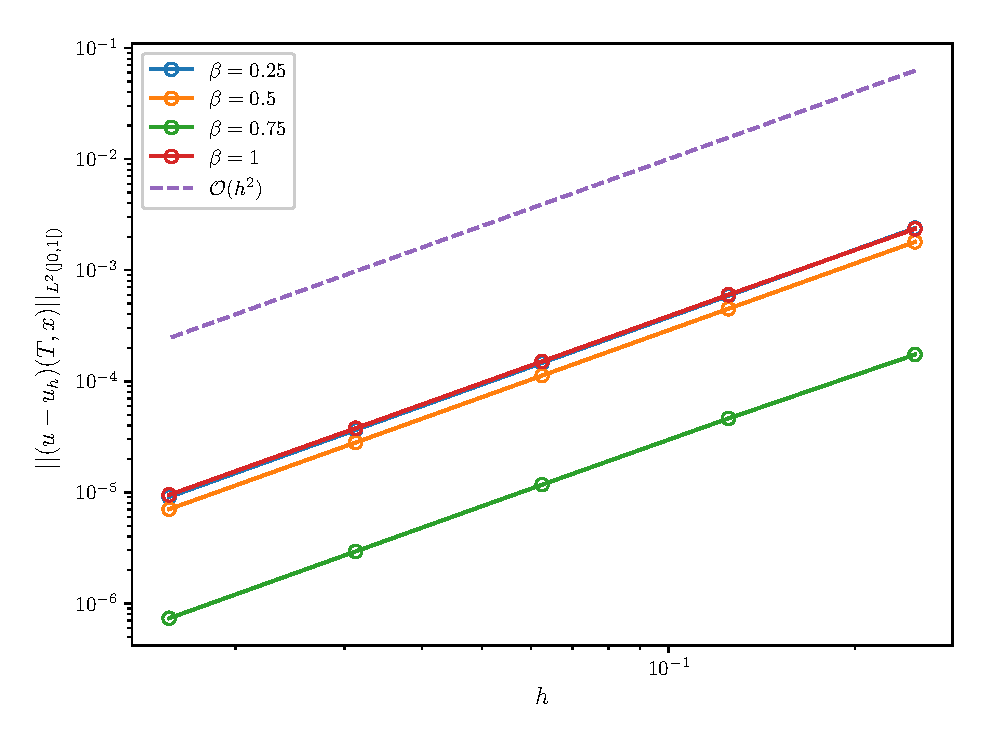
\includegraphics[width=1\linewidth]{figures/theta0/l2.eps}
  \caption{$\theta=0$, Explicit Euler.}
  \label{fig:sub1}
\end{subfigure}%
\begin{subfigure}{0.5\textwidth}
  \centering
  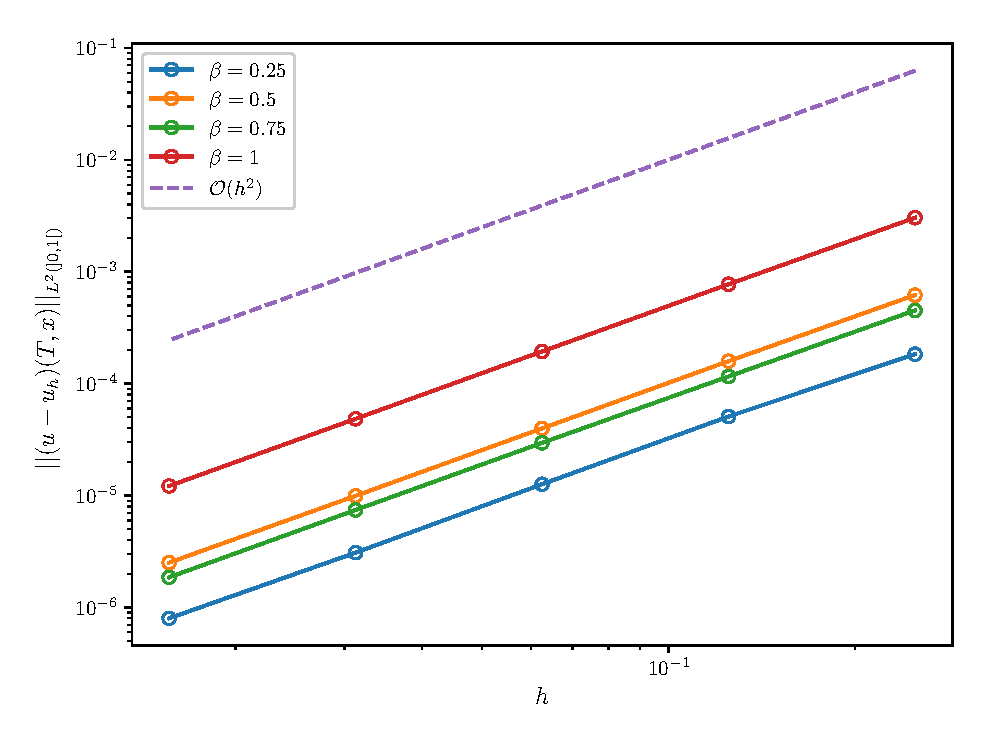
\includegraphics[width=1\linewidth]{figures/theta1o2/l2.eps}
  \caption{$\theta=1/2$, Crank--Nicolson.}
  \label{fig:sub2}
\end{subfigure} \\
\begin{subfigure}{0.5\textwidth}
  \centering
  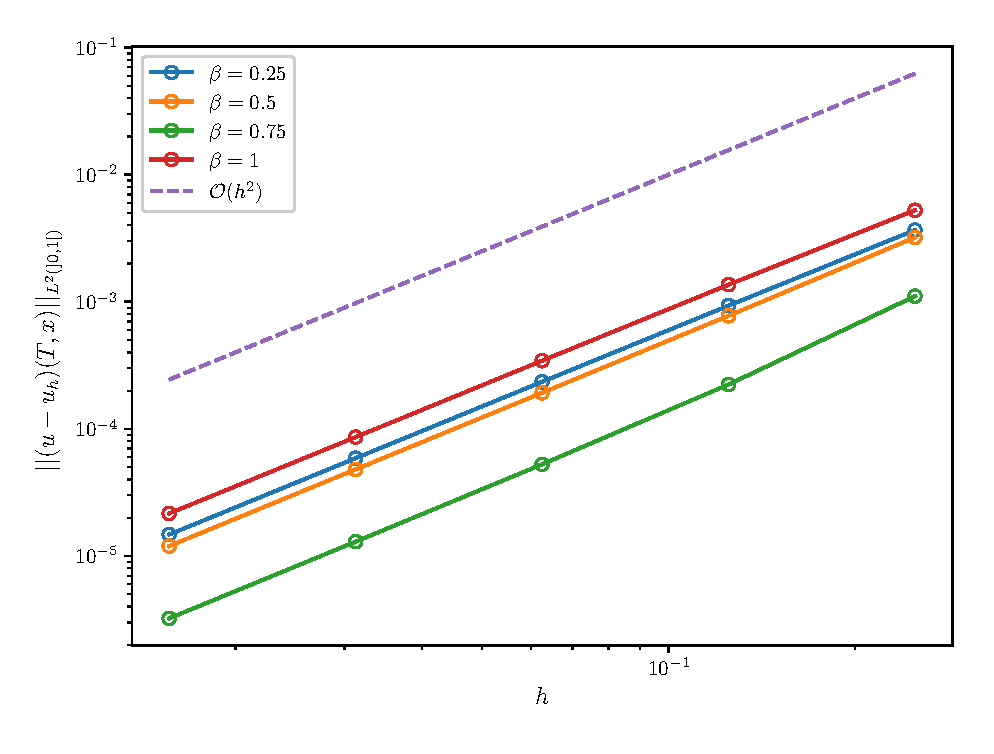
\includegraphics[width=\linewidth]{figures/theta1/l2.eps}
  \caption{$\theta = 1$, Implicit Euler.}
  \label{fig:sub2}
\end{subfigure}
\caption{The $L^2$-norm of the discretization error versus the mesh size $h$ for the Explicit Euler, Implicit Euler and the Crank--Nicolson schemes. }
\label{fig:sub2}
\end{figure}
\newpage
For linear finite elements, one can prove a second order convergence of the $L^2$ discretization error\cite{schwab}, in the non-fractional case. Indeed, the above plots exhibit quadratic $L^2$ convergence for all choices of $\beta$, in particular also for the non-fractional $\beta\in(0,1)$.  Moreover, we observe $\mathcal{O}(h^2)$ convergence of the discretization error in the $L^{\infty}$-norm.
\begin{figure}[h]
\centering
\begin{subfigure}{0.5\textwidth}
  \centering
  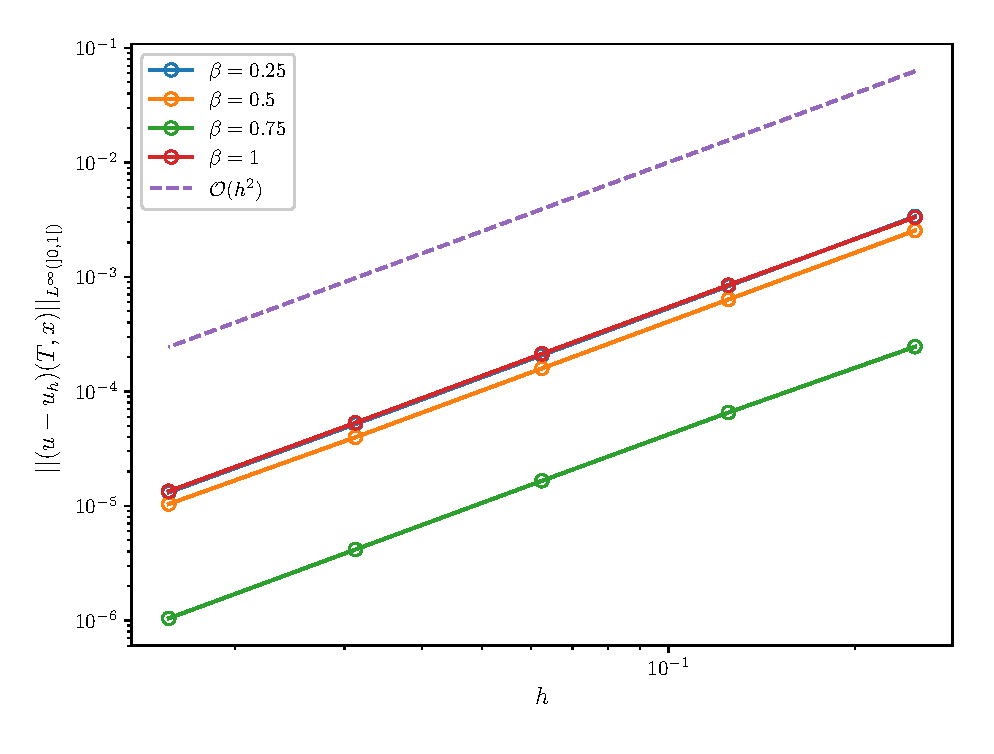
\includegraphics[width=1\linewidth]{figures/theta0/linf.eps}
  \caption{$\theta=0$, Explicit Euler.}
  \label{fig:sub1}
\end{subfigure}%
\begin{subfigure}{0.5\textwidth}
  \centering
  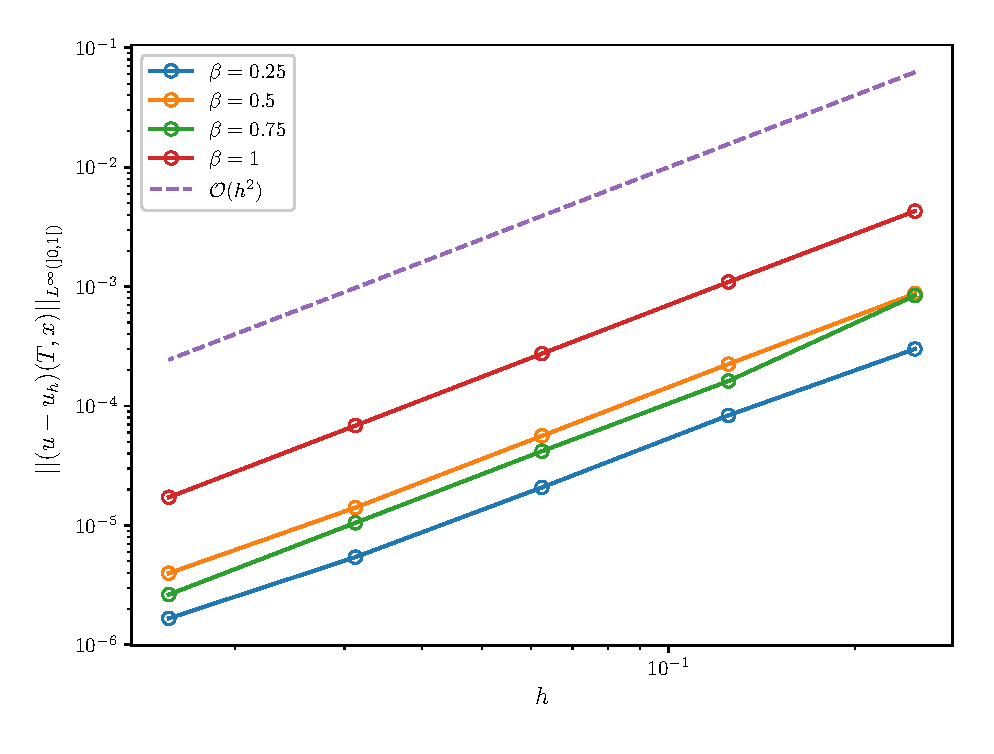
\includegraphics[width=1\linewidth]{figures/theta1o2/linf.eps}
  \caption{$\theta=1/2$, Crank--Nicolson.}
  \label{fig:sub2}
\end{subfigure} \\
\begin{subfigure}{0.5\textwidth}
  \centering
  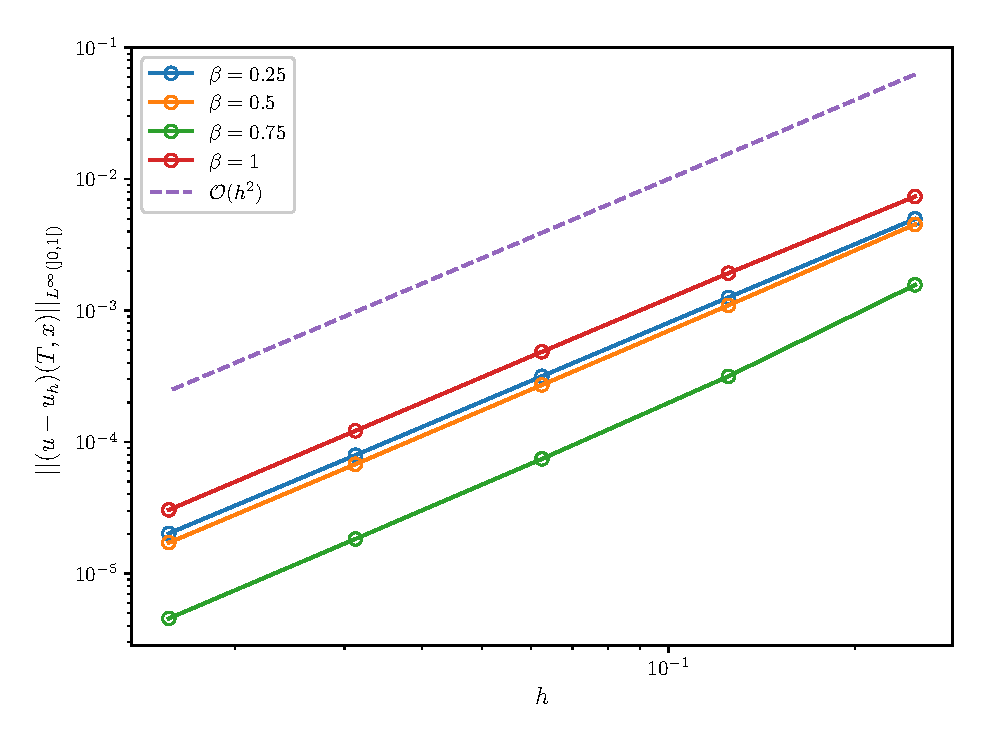
\includegraphics[width=\linewidth]{figures/theta1/linf.eps}
  \caption{$\theta = 1$, Implicit Euler.}
  \label{fig:sub2}
\end{subfigure}
\caption{The $L^{\infty}$-norm of the discretization error versus the mesh size $h$ for the Explicit Euler, Implicit Euler and the Crank--Nicolson schemes. }
\label{fig:sub2}
\end{figure}
Discretization error convergence results for other values of the parameter $\theta$ can be found in the appendix. \\
As a side note, in each iteration solving a linear system of equations is required and that provides a computational challenge because it makes the code slower. One possible solution is to parallelize the method \lstinline{std::for_each()} over several cores, where each core performs a summation of \eqref{sinc_quad} over a smaller number of steps, and that will speed-up the program.
% ------------------------------ 2D Fractional Heat Equation
\newpage
\subsection{The 2D Fractional Heat Equation}
Consider the 2D fractional heat equation on the unit square $\truncdom=(0,1)\times(0,1)$,
\begin{equation} \label{frac_heat_2D}
\begin{split} % \begin{split}
\partial_tv(t,\vx) + (-\Delta)^{1/2} v(t,\vx) = 0&, \quad  (t,\vx)\in(0,T]\times\truncdom, \\
v(0,\vx) = \vx_1(1-\vx_1)\vx_2(1-\vx_2)&, \quad \vx\in \truncdom, \\ 
v(t,\vx) = 0&, \quad (t,\vx) \in (0,T]\times\partial D.
\end{split}
\end{equation}
For $T=0.1$, figure \eqref{fig::md} shows the solution $v(T,\vx)$.

\begin{figure}[h]
\centering
  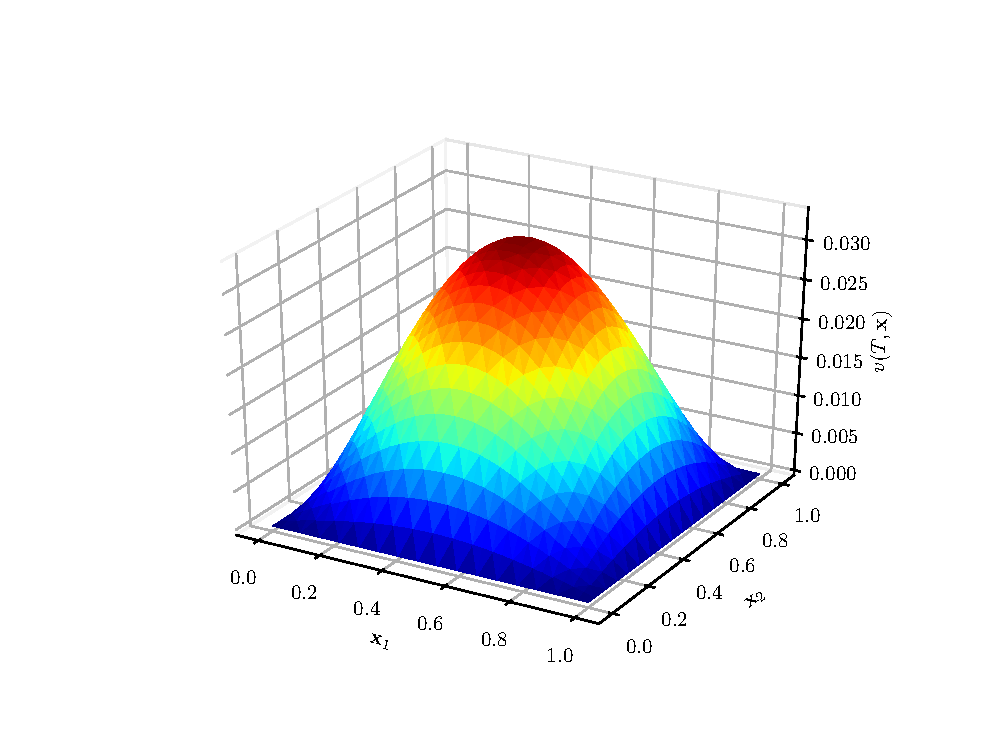
\includegraphics[width=0.8\linewidth]{figures/3d.eps}
  \caption{The solution of the 2D fractional heat equation.}
  \label{fig::md}
\end{figure}
% --------------------------- option pricing results
\subsection{An Application to Option Pricing}
We present numerical results corresponding to the pricing of European call and put options with continuous payoff funtions, and digital options with discontinuous payoffs. In the following, we denote by $(S_t)_{t\ge0}$ the price process of the underlying asset, $K$ the strike price and $T$ the option maturity. The payoff of the option is denoted by $g(s)$, where it is equal to $(s-K)^+$ for call options, $(K-s)^+$ for put options and $\mathbb{1}_{\{s>K\}}$ for digital options. For $\beta = 1/2$ (i.e, $\alpha=1$), the price process follows
\begin{equation} \label{sde_op}
\der S_t = rS_{t^{-}}\der t + \sigma\sqrt{S_{t^{-}}}\der L_t^{1},\quad S_0=s_0, 
\end{equation} 
where $(L_t^{1})_{t\ge 0}$ is an $1$-stable L\'{e}vy process, $r>0$ the risk-free interest rate and $\sigma>0$ the volatility. In this case, existence and uniqueness of solutions to \eqref{sde_op} follow immediately from the conditions discussed previously, with $\kappa(x) = rx$ and $\rho(x) =\sigma \sqrt{x}$. Indeed, $\kappa(x)$ is increasing and concave, $\kappa(0)=0, \int_0^{\infty}rx^{-1}\der x = \infty$ and $|rx-ry| = r|x-y| \le \kappa(|x-y|) \  \forall x,y\in\mathbb{R}.$ In addition to that, we have that $\rho(x)$ is increasing and concave, $\rho(0)=0$ and $\int_0^{\infty}(\sigma\sqrt{x})^{-1}\der x = \infty$. Finally, $|\sigma\sqrt{x}-\sigma\sqrt{y}| = \sigma|\sqrt{x}-\sqrt{y}| \le \sigma \sqrt{|x-y|} = \rho(|x-y|) \ \forall x,y\in\mathbb{R}.$ Indeed and assuming wlog.\ that $x\ge y>0$, squaring both sides of the latter inequality leads to
\begin{equation*}
x-2\sqrt{xy}+y \le x-y \implies 2\sqrt{xy} \ge 2y,
\end{equation*}
which follows from the assumption that $x\ge y.$
The infinitesimal generator $\mathcal{A}^1$ of the process $S$ is 
\begin{equation*}
\mathcal{A}^1 = rs\partial_s - \sigma\sqrt{s}(-\partial_{ss})^{1/2}.
\end{equation*}
The pricing parabolic PDE is then given by 
\begin{equation} \label{pricing_pde}
\begin{split} % \begin{split}
v_t(t,s) + \overbrace{\sigma \sqrt{s}(-\partial_{ss})^{1/2}v(t,s) - rs\partial_sv(t,s)}^{-\mathcal{A}^1v(t,s)} + rv(t,s) = 0&, \quad  (t,s)\in(0,T]\times (0,R), \\
v(0,s) = g(s)&, \quad s\in [0,R], \\ 
v_{\text{Call}}(t,0)=0,\ v_{\text{Digital}}(t,0)=0,\ v_{\text{Put}}(t,R) = 0&, \quad t \in (0,T].
\end{split}
\end{equation}
Call and digital options are approximated by down-and-out barrier options with barrier $H=0$, so that we impose homogeneous Dirichlet boundary conditions at $s=0$. On the other side, put options are approximated by up-and-out barrier options with barrier $H=R$, and so we impose homogeneous Dirichlet boundary conditions at $s=R$. In that case, the Poincar\'{e} inequality still holds since each of \{R\} and \{0\} has positive counting measure, and hence the whole theory of existence and uniqueness of weak solutions holds.\\ In the following, we fix $r=0.06, \sigma=0.6$ and $T=1$.

\begin{figure}[h]
\centering
\begin{subfigure}{0.5\textwidth}
  \centering
  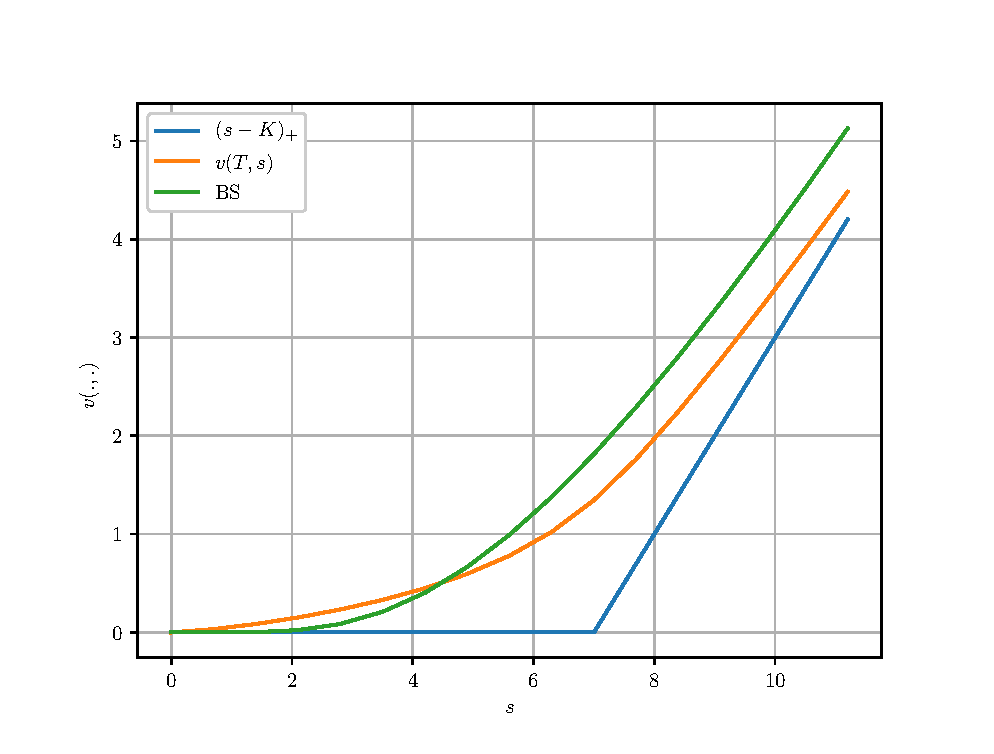
\includegraphics[width=1\linewidth]{figures/pricing/call_modi.eps}
  \caption{$K=7$, European call option.}
  \label{fig:sub1}
\end{subfigure}%
\begin{subfigure}{0.5\textwidth}
  \centering
  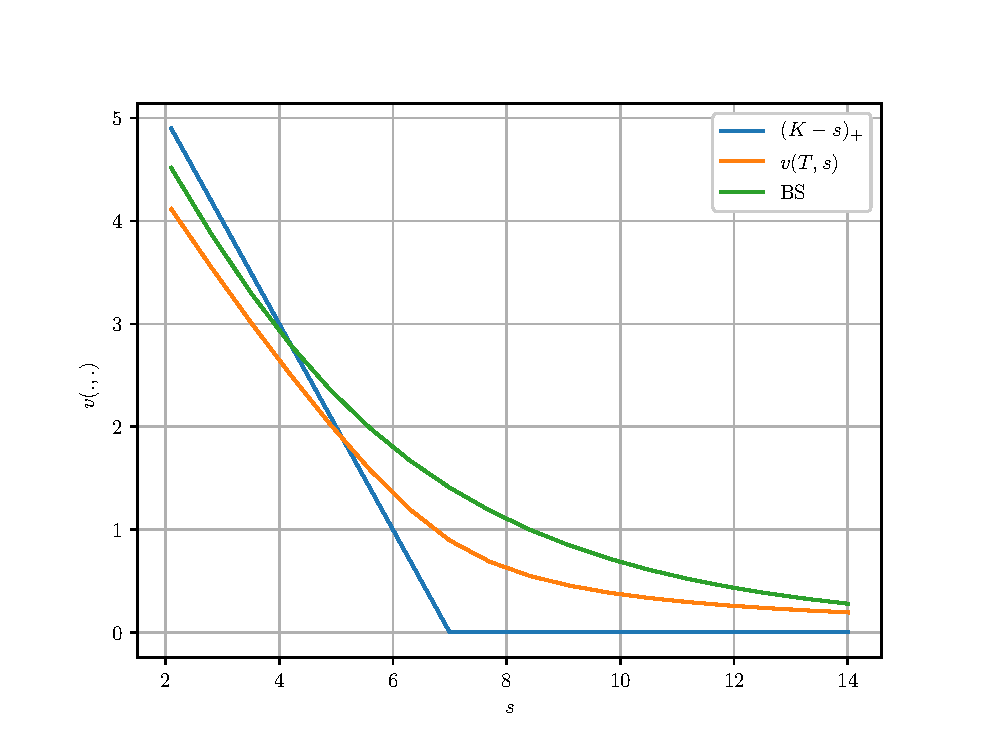
\includegraphics[width=\linewidth]{figures/pricing/put_modi.eps}
  \caption{$K= 7$, European put option.}
  \label{fig:sub2}
\end{subfigure} \\
\begin{subfigure}{0.5\textwidth}
  \centering
  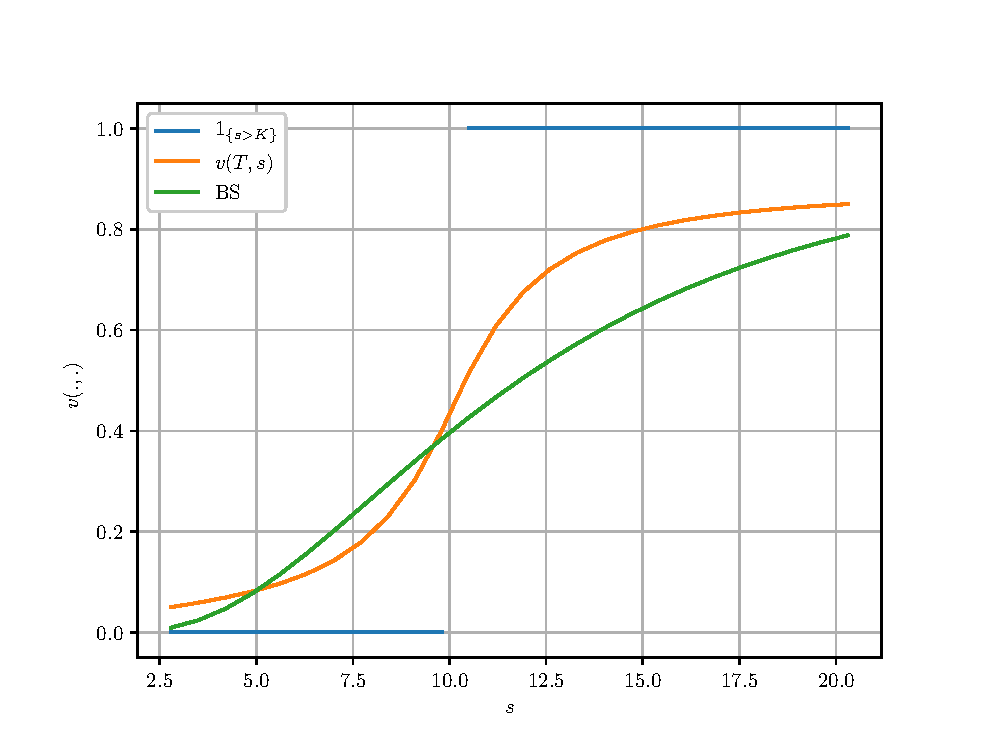
\includegraphics[width=1\linewidth]{figures/pricing/digital_modi.eps}
  \caption{$K=10$, European digital option.}
  \label{fig:sub1}
\end{subfigure}%
\caption{The price of European options under Feller--L\'{e}vy models (orange), together with the payoff (blue). For comparison: the corresponding price values in the Black-Scholes market (green).}
\label{fig:sub2}
\end{figure}


\newpage
% ------ Direct and Iterative Solvers Comparison
\subsection{Comparison of Direct and Iterative Solvers}
In this section we present a comparison in terms of computational time of the direct LU-factorization and the two iterative solvers, CGD and PCGD, all applied in case of the fractional heat equation \eqref{frac_heat_1D} and the pricing problem \eqref{pricing_pde}, for different number of mesh nodes $N$.  Table \eqref{table::time} summarizes the results, where the time is in seconds $(s)$. 
\begin{table}[h]
\centering
\begin{subtable}{0.5\textwidth}
  \centering
\begin{tabular}{|l|l|l|l|l|}
\hline
$N$        & 50   & 70    & 100   & 150                \\ \hline
SparseLU & 43.1 & 125.8 & 387.9 & \textgreater{}1000 \\ \hline
CGD      & 10.2 & 34.3 & 134.1 & 675             \\ \hline
PGCD     & 10.9 & 36.1 & 143.5 & 700.5        \\ \hline
\end{tabular}
  \caption{The fractional heat equation. }
  \label{fig:table1}
\end{subtable}%
\begin{subtable}{0.5\textwidth}
  \centering
\begin{tabular}{|l|l|l|l|l|}
\hline
$N$        & 50   & 70    & 80   & 100               \\ \hline
SparseLU & 73.4 & 186.06 & 288.7 & 602.2 \\ \hline
CGD      & 32.2 & 106.2 & 180.2 & 466.5           \\ \hline
PGCD     & 28.01 & 87.53 & 147.7 & 365.2        \\ \hline
\end{tabular}
  \caption{The pricing problem.}
  \label{fig:tabl2}
\end{subtable}%
\caption{Computational time comparison for the LU-factorization, CGD and PCGD.}
\label{table::time}
\end{table}
For the fractional heat equation, the CGD always outperforms the direct LU solver, however the PCGD performs slightly worse than the CGD, but better than the direct LU solver. As for the pricing problem, the CGD also outperforms the direct LU solver and the same goes for the PCGD, but we notice that the preconditioning improves the computational time as opposed to the case of the fractional heat equation. This can be given an intuitive explanation using the following plot.
\begin{figure}[h]
  \centering
  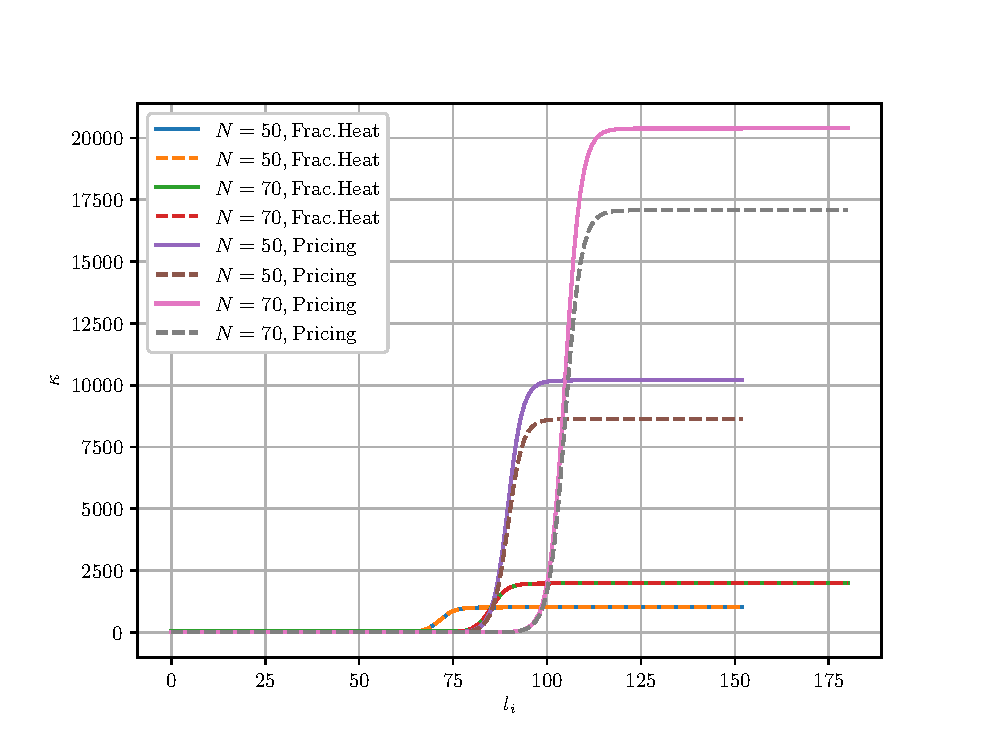
\includegraphics[width=0.5\linewidth]{figures/kappa.eps}
  \caption{Evolution of the condition number $\kappa$ for the case of the fractional heat equation and the pricing problem for N=50 and N=70. The solid lines correspond to the CGD and the dashed lines correspond to the PCGD.}
  \label{fig:kappa}
\end{figure}\\
The condition number of a matrix $\mathbf{X}$, $\kappa(\mathbf{X})$ is defined by
\begin{equation*}
\kappa(\mathbf{X}) = \frac{\sigma_{\text{max}}}{\sigma_{\text{min}}},
\end{equation*}
where $\sigma$ is a singular value of the matrix $\mathbf{X}$. The solid lines in the plot represent the condition number $\kappa(\myexp^{2lk}\stiff+\mass)$ for all $l$ in the sum in equation \eqref{sinc_quad}, where the iterative solver is applied. On the other side, the dashed lines correspond to the condition number after diagonal preconditioning, that is $\kappa(\mathbf{D}^{-1}(\myexp^{2lk}\stiff+\mass))$ where $\mathbf{D}=\text{diag}(\myexp^{2lk}\stiff+\mass)$. The following code shows how to calculate the condition number of a matrix in C++ Eigen.
\begin{lstlisting}[caption={Condition number computation in C++.}] 
double conditionNumber(Eigen::MatrixXd& A){
	Eigen::SVDJacobi<Eigen::MatrixXd> svd(A); 
	Eigen::VectorXd singularValues = svd.singularValues();
	return singularValues(0) / singularValues(singularValues.size()-1); 
}
\end{lstlisting}
Clearly, we do not get any improvement in the condition number after preconditioning in the case of the fractional heat equation, and that is why the PCGD performs worse in that case. More precisely, we do not get faster convergence of the iterative solver while we are adding the computation overhead of the preconditioning. In contrast, we can see from the plot that the condition number decreases after preconditioning in the pricing problem, and that leads to an improvement in the computational time, gaining a faster convergence that is dominating the computation overhead of the preconditioning, and that explain the corresponding results in table \eqref{table::time}.


% --------------------------- Conclusion
\newpage
\section{Conclusion}
In this project, we have implemented the finite element method for option pricing under Feller--L\'{e}vy models, where the fractional Laplacian operator shows up in the parabolic partial differential equation that governs the price process. The finite element approximation of the latter operator has been established using the sinc quadrature. In the finite element solver, solving a linear system at each step has been done using the conjugate gradient descent iterative method, and that is due to the fact that the finite element matrix approximation matrix of the fractional Laplacian is not known explicitly and hence cannot be inverted. However, the sinc matrix approximation of the fractional Laplacian raised a computational challenge, namely the computationally expensive sum in \eqref{sinc_quad} and future work may be done by parallelizing the latter sum to speed up the program. \\
After highlighting the C++ object-oriented implementation of the finite element method, we showed  for the case of the fractional 1D heat equation an empirical second order convergence of the discretization error in the $L^2$ and $L^{\infty}$ norms that was in accordance with the theoretical rates of convergence presented for the non-fractional case in\cite{schwab}. In addition to that, the linear system showing up in the equation of the sinc matrix has been solved using three different direct and iterative methods, namely the LU-factorization technique, and the conjugate gradient descent with and without preconditioning. We have shown that iterative methods speed up the program especially when the number of mesh nodes is large enough, however the preconditioning seems to be of importance depending on the nature of the problem.

% --------------------------- References
\newpage
\bibliography{bibfile.bib}
\bibliographystyle{acm}

% --------------------------- Appendix
\newpage
\section{Appendix}
\subsection{Additional Convergence Results}
The following plots show the second order convergence of the discretization error in the $L^2$ and $L^{\infty}$ norms for $\theta \in \{1/4, 3/4 \}$.
\begin{figure}[h]
\centering
\begin{subfigure}{0.5\textwidth}
  \centering
  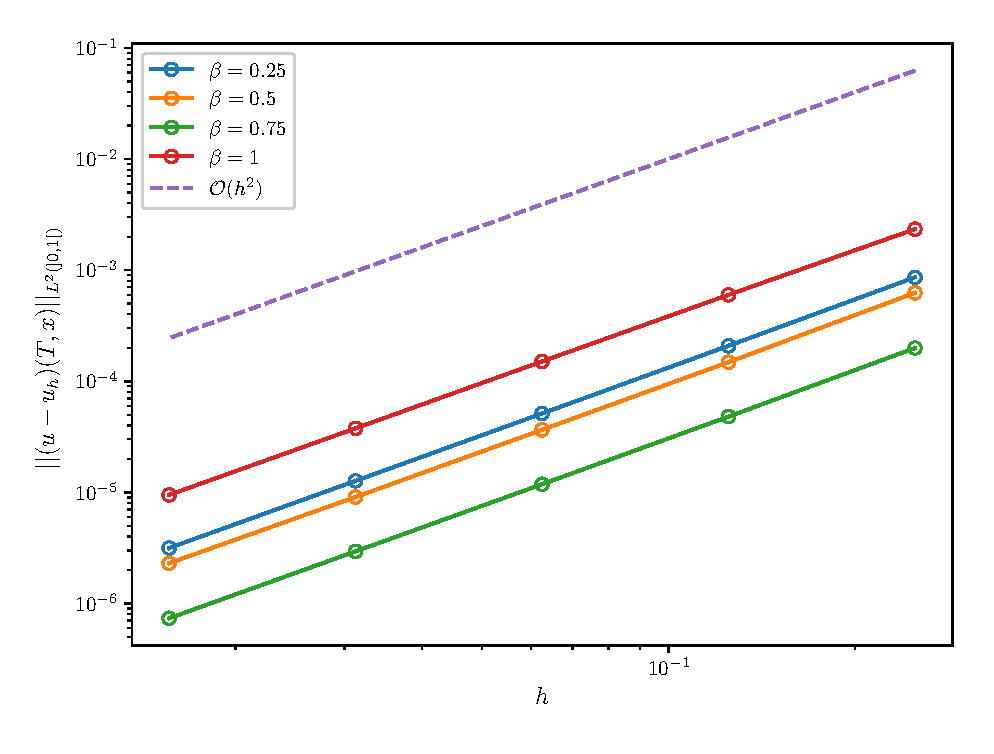
\includegraphics[width=1\linewidth]{figures/theta1o4/l2.eps}
  \caption{$\theta=1/4$.}
  \label{fig:sub1}
\end{subfigure}%
\begin{subfigure}{0.5\textwidth}
  \centering
  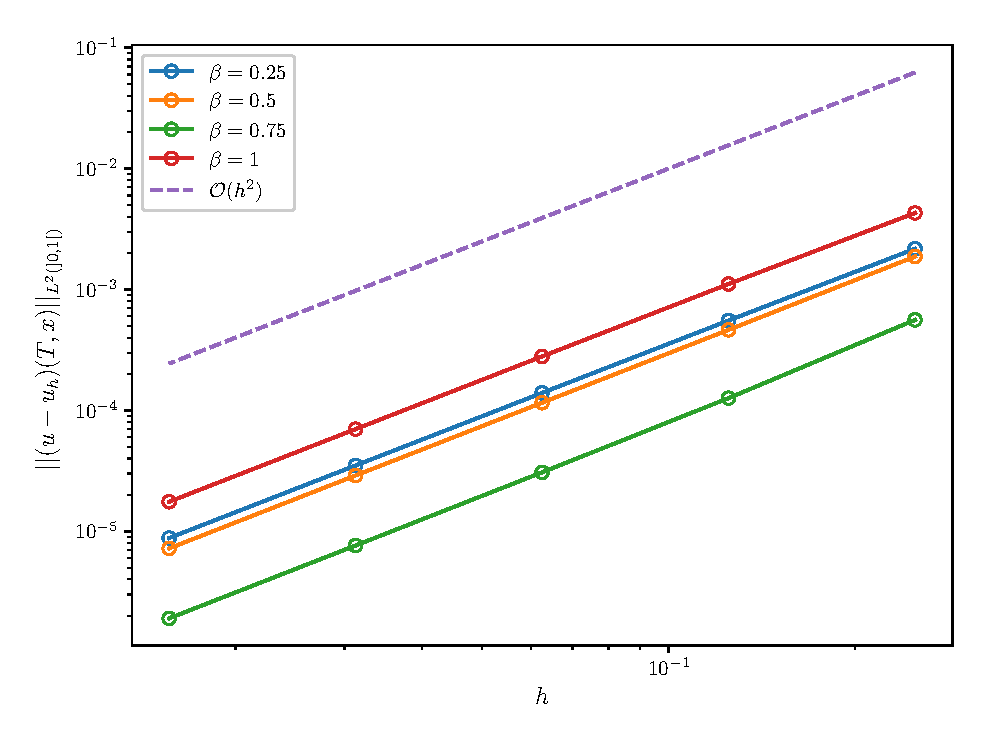
\includegraphics[width=1\linewidth]{figures/theta3o4/l2.eps}
  \caption{$\theta=3/4$.}
  \label{fig:sub2}
\end{subfigure}
\caption{The $L^{2}$-norm of the discretization error versus the mesh size $h$ for $\theta \in \{1/4, 3/4 \}$. }
\label{fig:sub2}
\end{figure}

\begin{figure}[h]
\centering
\begin{subfigure}{0.5\textwidth}
  \centering
  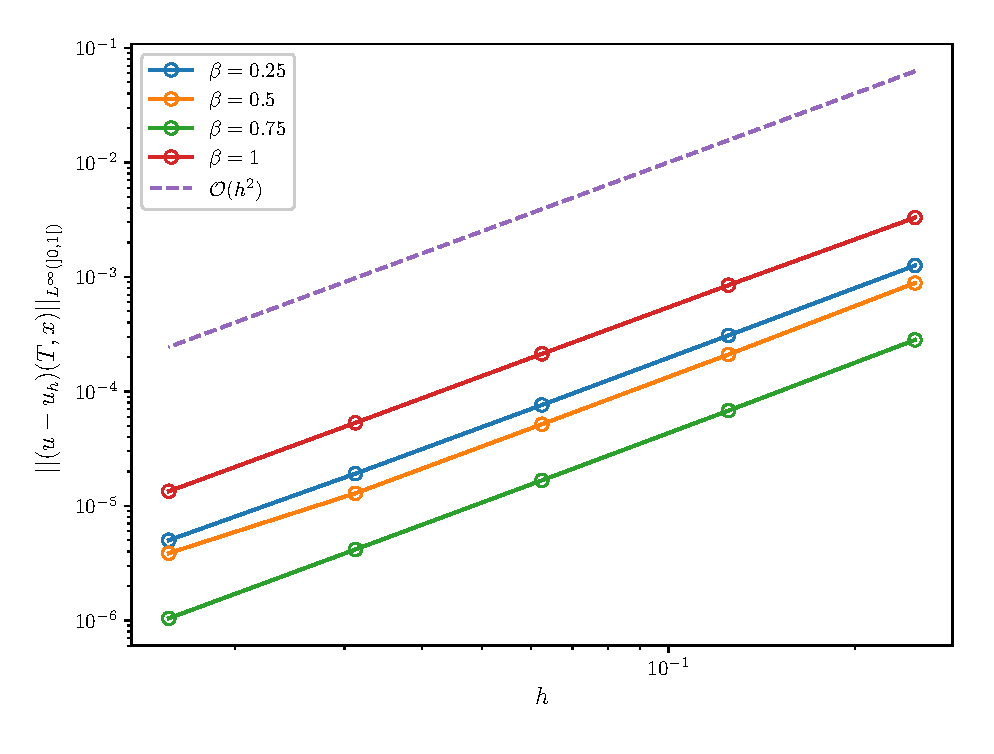
\includegraphics[width=1\linewidth]{figures/theta1o4/linf.eps}
  \caption{$\theta=1/4$.}
  \label{fig:sub1}
\end{subfigure}%
\begin{subfigure}{0.5\textwidth}
  \centering
  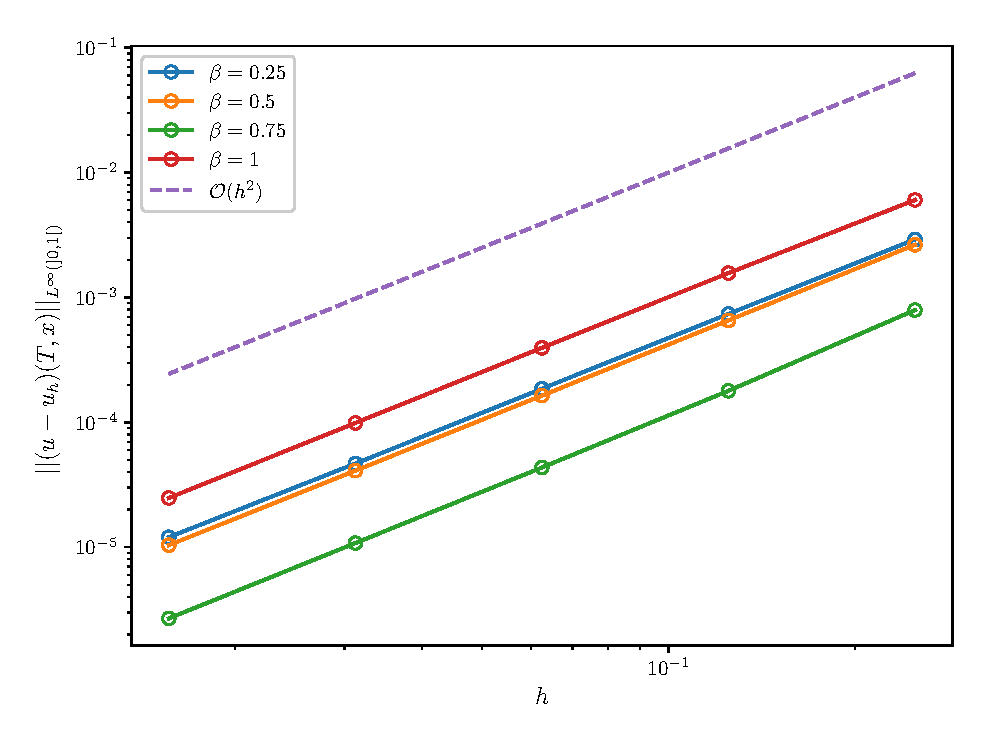
\includegraphics[width=1\linewidth]{figures/theta3o4/linf.eps}
  \caption{$\theta=3/4$.}
  \label{fig:sub2}
\end{subfigure}
\caption{The $L^{\infty}$-norm of the discretization error versus the mesh size $h$ for $\theta \in \{1/4, 3/4 \}$. }
\label{fig:sub2}
\end{figure}

\newpage
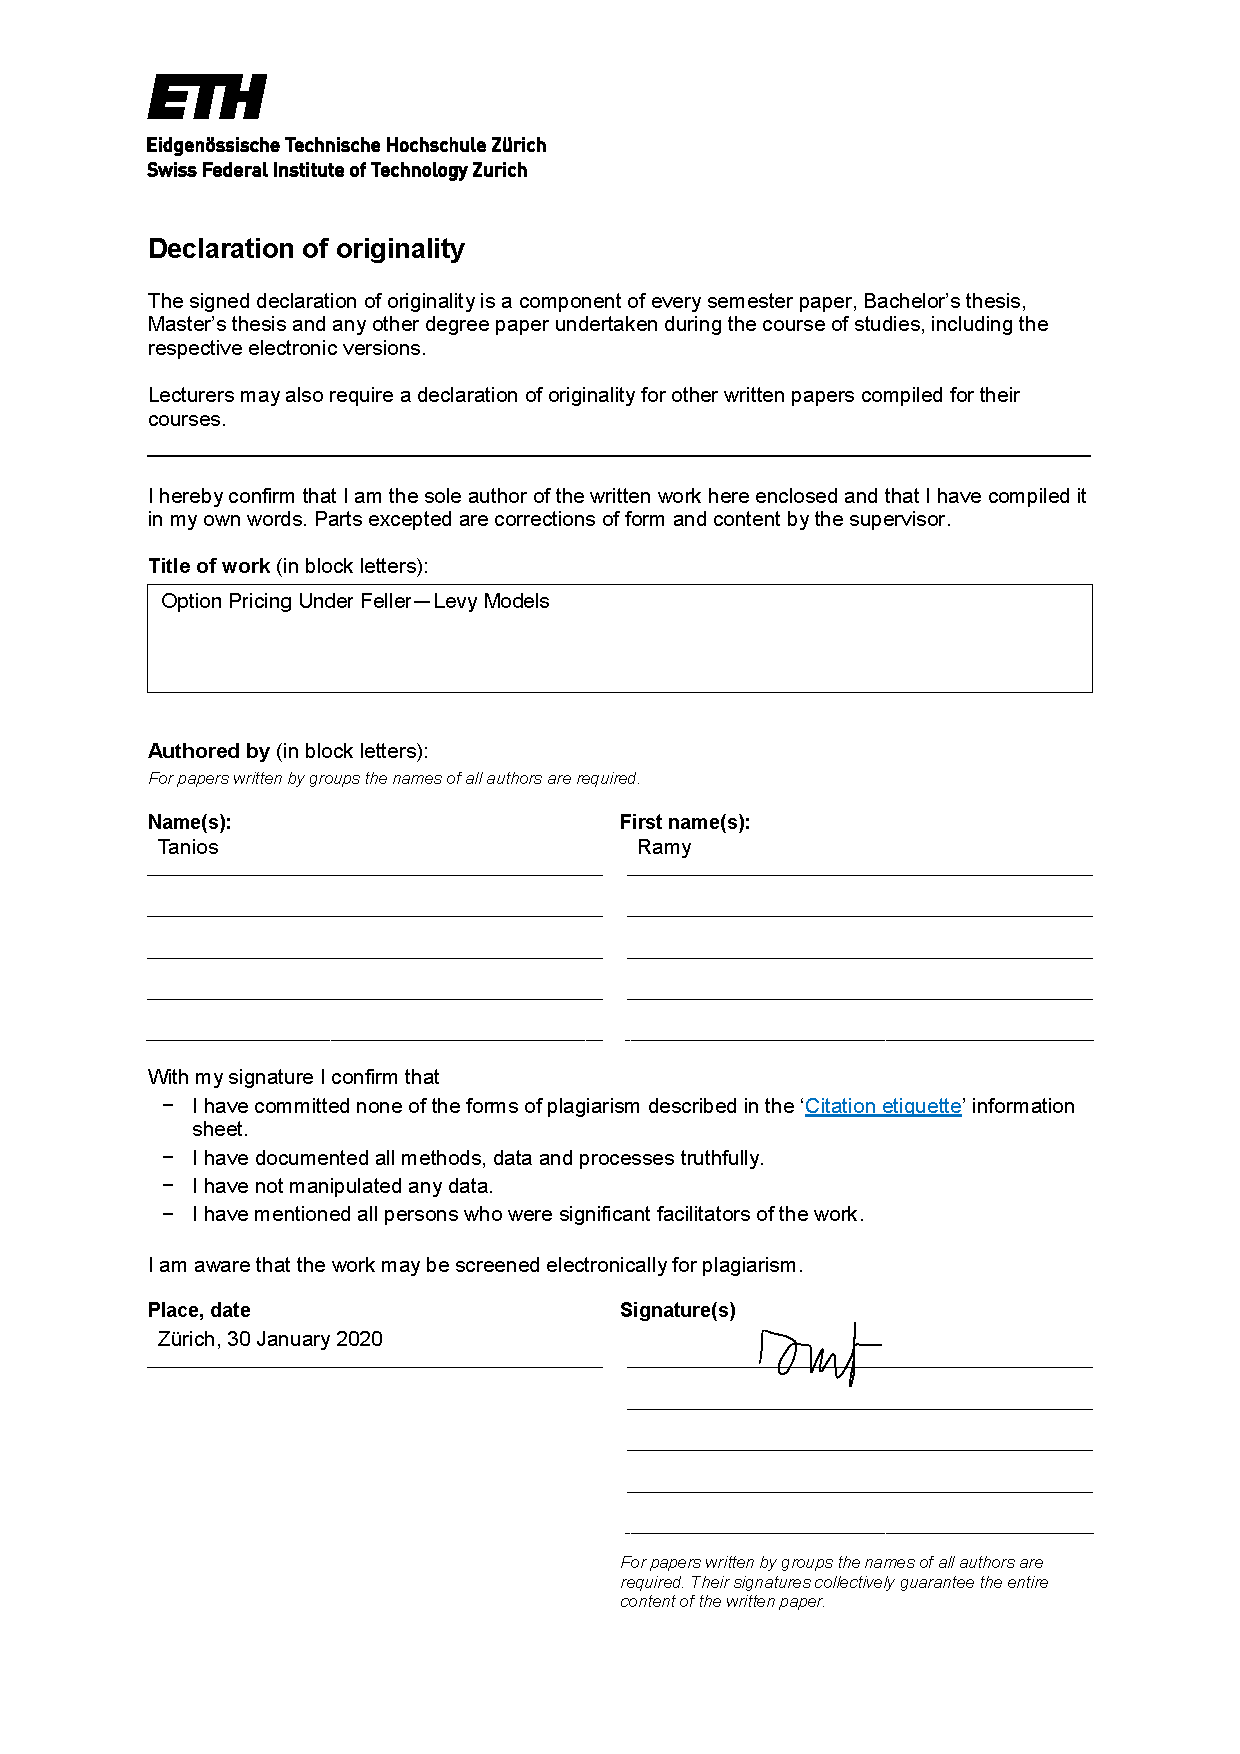
\includepdf[pages=-,pagecommand={},width=\textwidth]{originality}


\end{document}
%----------------------------------------------------------------------------------------
%	DONE
%----------------------------------------------------------------------------------------
